\chapter{Background}
\label{ch:Background}

L'incremento di quantità, la possibilità di ridurre rischi e permettere di avere una previsione sulle possibili tendenze di mercato, migliori prestazioni in ambito dei processi decisionale e la presa di coscienza da parte delle aziende su tutti i benefici acquisibili migrando il proprio sistema in un orientamento data-driven. Questi sono solo alcune delle motivazioni che hanno portato i dati a incrementare il proprio valore e importanza all'interno del mondo. Per questa ragione, con il tempo sono state diverse le tecnologie e i processi applicati a quest'ultimi per poter migliorare la loro gestione ed efficienza (e di conseguenza il valore da loro ricavabile). I più importanti tra questi sono i \textit{Big Data}, i \textit{Data Warehouse} e l'\textit{Analisi dei dati}.

\section{I Big Data}

Come accennato in precedenza le esigenze di salvataggio e gestione dei dati sono diventate sempre più importati, proprio per tale motivo ha guadagnato importanza a sua volta anche il mondo dei \textit{Big Data}. Ovvero il campo emergente in cui l'evoluzione del mondo e della sua tecnologia offre nuovi modi per recuperare il valore dalla marea di informazioni generate. La capacità di gestire efficientemente le informazioni e di estrarre conoscenza da quest'ultime è diventato un vantaggio sempre più importante a cui ogni azienda aspira. Di conseguenza, molte compagnie si stanno ponendo come obiettivotanto da farlo diventare anche il proprio core business, la capacità di raccogliere e analizzare i dati, così da ricavarne il maggior numero di informazioni utili possibili. L'adozione della tecnologia dei Big Data nell'ambito delle compagnie non può più definirsi una scelta opzionale, bensì una necessità obbligata per sopravvivere ed ottenere un vantaggio competitivo \cite{new_horizon_for_a_data_driven_economy}.

Ciò è dovuto al fatto che senza informazioni che possano considerarsi adeguate (definite tali poiché consentirebbero di svolgere scelte corrette dettate dalla conoscenza ricavata dalla lettura di tali dati), difficilmente si potrebbe ottenere una strategia vincente. I Big Data sono ciò che permette di svolgere questo compito al meglio, trattandosi di beni da cui è possibile estrarre moltissime informazioni che poi potranno essere impiegate per prendere le decisioni nel miglior stato di conoscenza possibile.

Ad avvalorare tali affermazioni, la Acumen Research Consulting (ARC), fornitore globale di servizi di market intelligence e di consulenza per le tecnologie dell'informazione, ha svolto un analisi del mercato dei Big Data relativo al 2021. La Figura \ref{fig:Global-Big-Data-Market} mostra i risultati che hanno attribuito ai Big Data un valore complessivo di 165,5 miliardi di dollari. Inoltre, a seguito di approfonditi studi, è stato previsto un incremento del valore fino a 473,6 miliardi nel 2030 dovuto ad un CAGR\footnote{Il \textit{Compound Annual Growth Rate} (\textit{CAGR}), o \textit{Tasso di crescita annuale composto}, corrisponde alla crescita percentuale media di una grandezza in un lasso di tempo.} del 12,7\%\footnote{\textit{URL Fonte}: https://www.acumenresearchandconsulting.com/big-data-market}.

\begin{figure}[H]
    \centering
    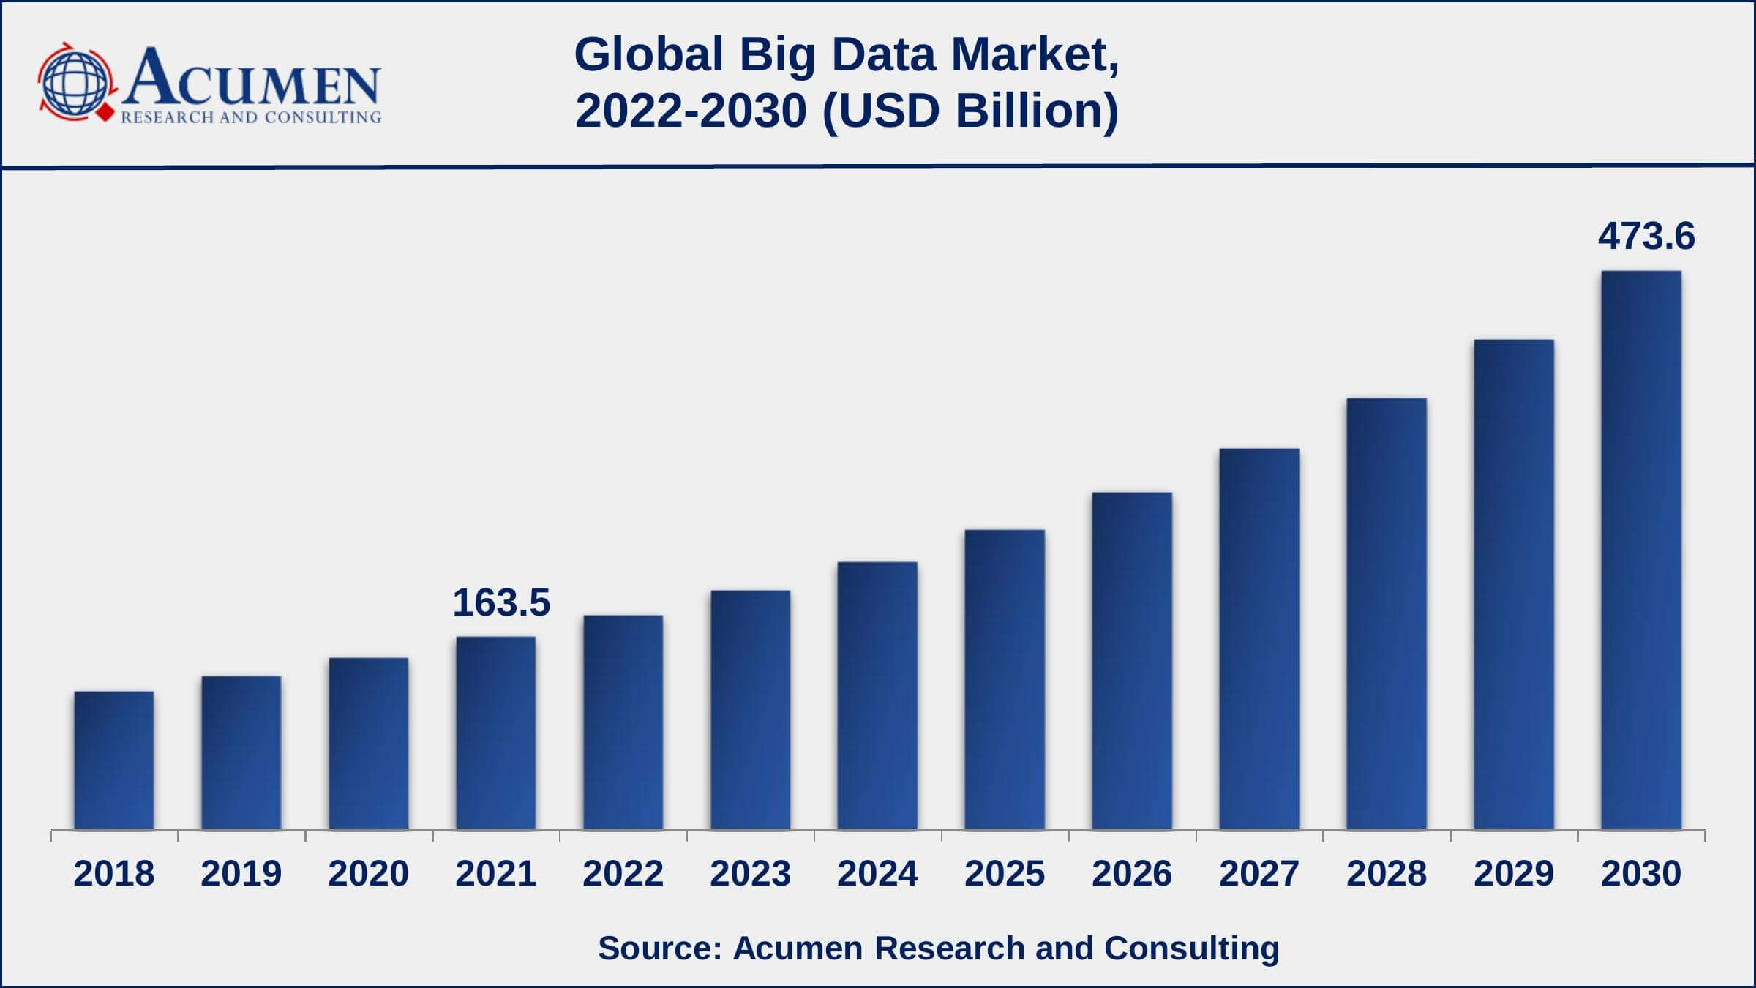
\includegraphics[width=0.7\linewidth]{figure/capitolo_2/Global-Big-Data-Market.pdf}
    \caption{Valore del mercato globale dei Big Data}
    \label{fig:Global-Big-Data-Market}
\end{figure}

\subsection{Definizione di ``Big Data''}

Poiché il dominio dei Big Data è molto eterogeneo, non è ancora possibile evidenziare l'esistenza di una definizione univoca capace di rappresentare tutti i contesti di utilizzo. Per garantire un'analisi completa, abbiamo esaminato le definizioni più pertinenti seguendo le linee guida proposte da Garousi et al. \cite{GAROUSI}. Questo studio ha coinvolto l'esame sia della letteratura ``grigia'' che di quella ``bianca'', includendo sia le pubblicazioni scientifiche che quelle non pubblicate.

Facendo ciò ci è stato possibile comprendere come, anche senza un vero e proprio riferimento ad una definizione ufficiale, molti sono stati i riferimenti eterogenei al mondo dei Big Data. Per poter capire effettivamente cosa siano i Big Data bisogna quindi adoperare una definizione ufficiale, purtroppo però ad oggi non è stata ancora creata. Per questo motivo, di seguito sono riportate le più rilevanti e significative definizioni pubblicate nel tempo.

\begin{longtable}{|p{11cm}|p{3cm}|}
    \caption{Definizioni di Big Data} \\
    \hline
    \textbf{Definizione} & \textbf{Autore} \\
    \hline
    \endfirsthead
    «I Big Data sono risorse informative ad alto volume, alta velocità e/o alta varietà che richiedono nuove forme di elaborazione per consentire una migliore presa di decisioni, scoprire nuove intuizioni e ottimizzare i processi.» 
    & Laney Doug (2001) \cite{laney_3d_data_management}\\
    \hline
    «Quando le dimensioni dei dati stessi diventano parte del problema e le tecniche tradizionali per lavorare con i dati perdono efficacia.» 
    & Mike Loukides (2010) \cite{loukides_data_science}\\
    \hline
    «Dati le cui dimensioni ci costringono a guardare oltre i metodi collaudati e consolidati in quel momento.» 
    & Jacobs Adam (2009) \cite{jacobs_big_data}\\
    \hline
    «Le tecnologie Big Data rappresentano una nuova generazione di tecnologie e architetture progettate per estrarre valore in modo economico da volumi molto ampi di dati di varie tipologie, consentendo la cattura ad alta velocità, la scoperta e/o l'analisi.» 
    & IDC (2011) \cite{idc_big_data}\\
    \hline
    «I Big Data sono un insieme enorme di dati complessi che richiedono metodologie, strumenti e competenze atte a gestirli, processarli, estrarli ed analizzarli.» 
    & Elisa Iandiorio (2021) \cite{iandorio_big_data}\\
    \hline
    «Una raccolta di insiemi di dati grandi e complessi che possono essere elaborati solo con difficoltà utilizzando strumenti di gestione di database normalmente disponibili.» 
    & Mike 2.0. (2014) \cite{mike_big_data}\\
    \hline
    «Il termine “Big Data” comprende l'uso di tecniche per catturare, elaborare, analizzare e visualizzare potenzialmente grandi insiemi di dati in un periodo di tempo ragionevole non accessibile alle tecnologie informatiche standard.» 
    & NESSI (2012) \cite{nessi_big_data}\\
    \hline
    «I Big Data di solito includono insiemi di dati di dimensioni oltre la capacità dei comuni strumenti software di recuperare, pulire, gestire ed elaborare dati entro un tempo trascorso tollerabile.» 
    & Risorsa Web (2023) \cite{wikipedia_big_data}\\
    \hline
    «Insiemi di dati estremamente grandi che possono essere analizzati computazionalmente per rivelare modelli, tendenze e associazioni, specialmente in relazione al comportamento umano e alle interazioni.» 
    & Google Dictionary (2023) \cite{google_big_data}\\
    \hline
    «Definiamo i Big Data come un fenomeno culturale, tecnologico e accademico che si basa sull'interazione tra: (1) Tecnologia: massimizzare la potenza di calcolo e l'accuratezza algoritmica per raccogliere, analizzare, collegare e confrontare grandi insiemi di dati. (2) Analisi: trarre vantaggio da grandi insiemi di dati per identificare modelli al fine di formulare affermazioni economiche, sociali, tecniche e legali. (3) Mitologia: la diffusa convinzione che grandi insiemi di dati offrano un livello superiore di intelligenza e conoscenza che può generare intuizioni che in passato erano impossibili, con l'aura di verità, oggettività e precisione.» 
    & Danah Boyd, Kate Crawford (2012) \cite{routledge_big_data}\\
    \hline
\end{longtable}

\begin{figure}[H]
    \centering
    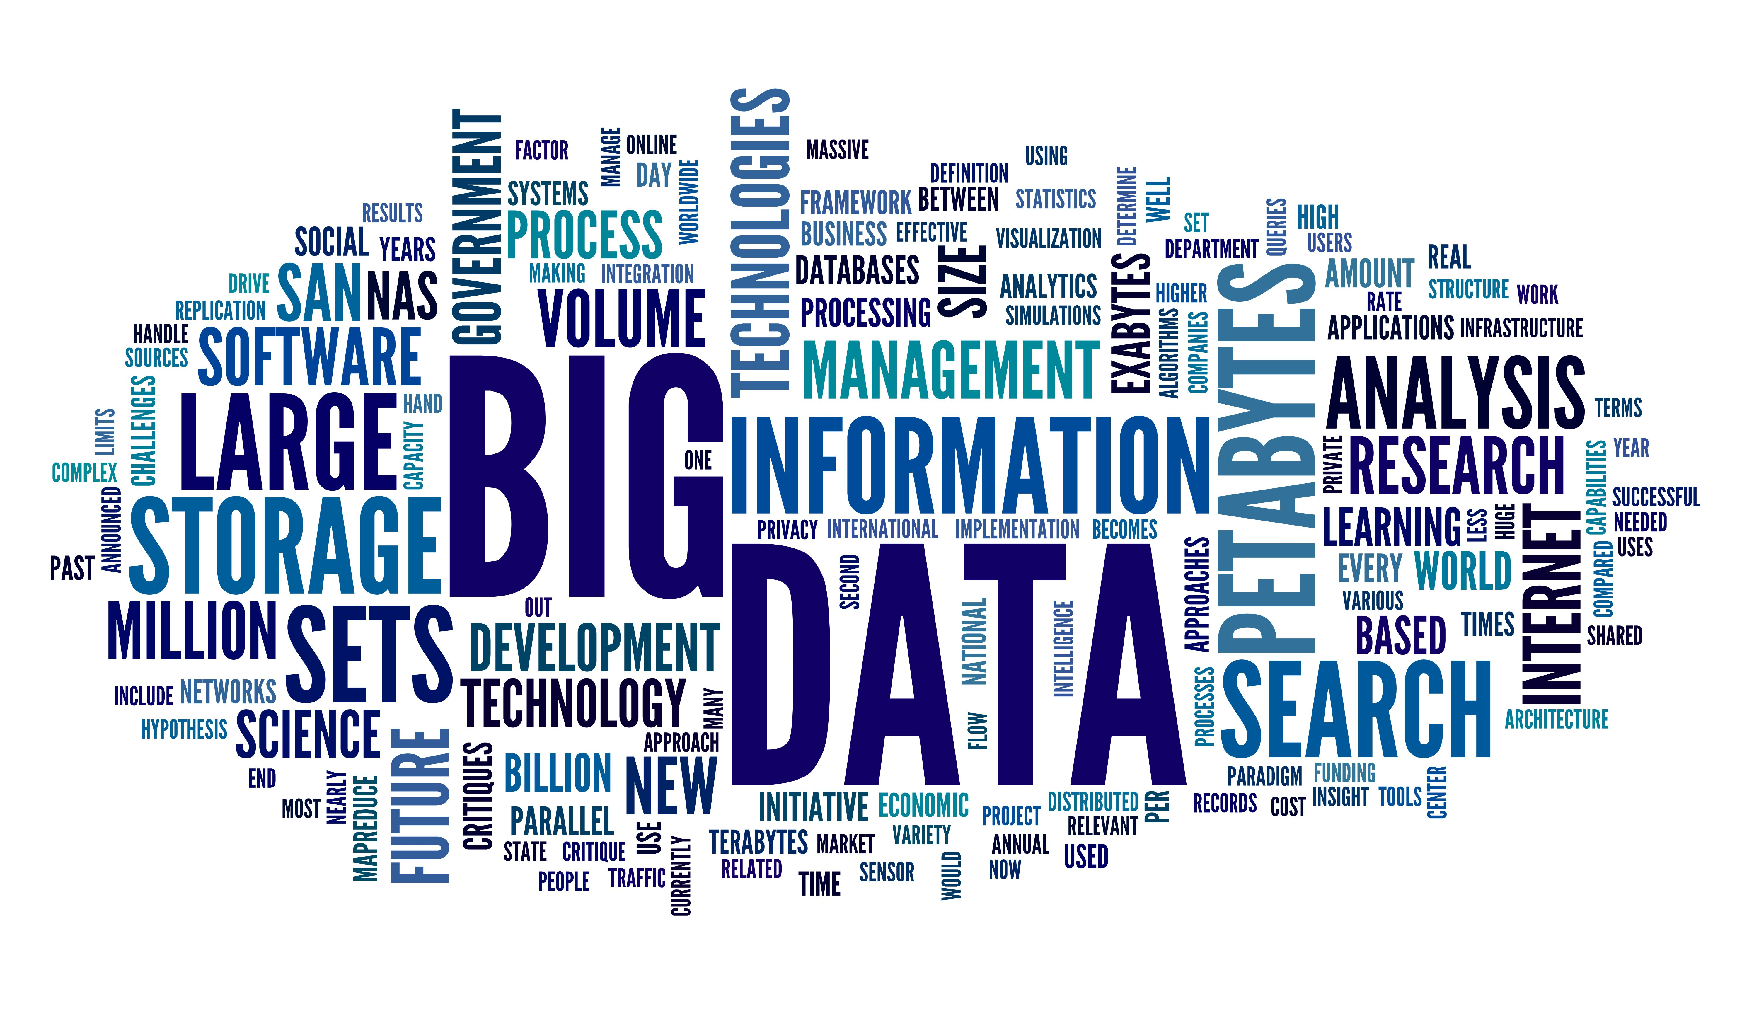
\includegraphics[width=0.8\linewidth]{figure/capitolo_2/Big_Data.pdf}
    \caption{I Big Data}
    \label{fig:Big_Data}
\end{figure}

Naturalmente, queste sono solamente le definizioni identificate come le più rilevanti o anche discordanti tra loro, ma non tutte quelle esistenti. Ciò permette di apprendere come, per quanto non esista una definizione standard, tra tutte quelle esistenti create arbitrariamente dagli studiosi, a seguito di ampie ricerche, siano presenti delle caratteristiche comuni --come visibile nella rappresentazione riportata nella Figura \ref{fig:Big_Data}\footnote{\textit{URL Figura}: https://tinyurl.com/48b6ymvf}. Perciò, da tali tratti distintivi è possibile affermare che:

\begin{center}
\textit{Il termine Big Data fa riferimento ad un processo adoperante un insieme di dati, anche eterogenei fra loro, la cui dimensione, complessità e velocità di acquisizione ne rendono difficile la gestione, in tempi accettabili, attraverso strumenti e processi tradizionali; tuttavia, grazie ad apposite risorse (personale, hardware e software) tale processo permette di svolgere una gestione ed analisi dei dati tale da ricavare valore da questi in quantità, qualità e tempistiche prima impensabili.}
\end{center}

Quindi, è possibile semplificare il concetto dicendo che con l'espressione “Big Data” si indica la raccolta di una grande mole di dati digitali che, per acquisire valore, richiedono l'utilizzo di specifiche infrastrutture, metodologie di gestione e modelli di analisi. Come è possibile dedurre, il motivo per cui non è stato possibile creare una definizione specifica e che potesse essere assoluta è dovuto al concetto stesso di Big Data. Esso dipende principalmente dal fatto che si parla di una gestione ed analisi di dati che non sarebbe applicabile con tecnologie comuni, con l'evoluzione di quest'ultime dovute al passare degli anni le capacità di elaborazioni migliorerebbero e quindi ciò che era considerato Big Data in passato potrebbe non essere considerato tale oggi o in futuro. Proprio per questo motivo la definizione di Big Data deve essere generica, relativa e dinamica data la sua possibile continua evoluzione.

Sicuramente sentendo le parole “Big Data” una delle prime associazioni che si hanno nella propria mente è quella di un grande volume di dati, tuttavia se si volesse conoscere la quantità precisa per comprendere quando effettivamente si stia parlando di Big Data ciò non sarebbe possibile per due motivi:

\begin{itemize}
    \item sono definiti “grandi” non solo per il loro volume, ma anche per la varietà e la complessità che li contraddistingue;
    \item per lo stesso motivo del “problema” che affligge la definizione del termine Big Data, non è possibile quantificare il volume minimo per parlare di Big Data poiché le dimensioni che si hanno al giorno d'oggi, come abbiamo potuto apprendere in precedenza, non sono paragonabili a quelle passate o future.
\end{itemize}

\subsection{Caratteristiche}

A seguito del proprio studio sul fenomeno dei Big Data, Doug Laney elaborò un nuovo modello in grado di definire quali fossero le loro caratteristiche. Prese il nome di “\textbf{Modello delle 3V}”, poiché pone i 3 concetti di \textit{Volume, Velocità e Varietà} alla base della definizione di Big Data. Col passare degli anni e con l'evoluzione del fenomeno tale modello è stato integrato con altre quattro proprietà in grado di definire e interpretare ancor di più nello specifico le caratteristiche di ogni dato, ovvero \textit{Valore, Veridicità, Valenza e Visualizzazione}. (È importante precisare che risulta difficile isolare le singole caratteristiche poiché esiste una forte legame tra di loro.) Di seguito sono riportate le definizioni delle caratteristiche elencate \cite{agcom_big_data}.
\begin{itemize}
    \item \textbf{Volume} (\textit{Volume}). Il volume rappresenta la caratteristica che più facilmente si può accostare ai Big Data; però come detto in precedenza numerosi sono stati gli studi che cercano di misurare tale caratteristica, tuttavia è stata riscontrata l'impossibilità di conoscerne il preciso ammontare.
    \item \textbf{Varietà} (\textit{Variety}). La varietà fa riferimento all'eterogeneità delle fonti sorgenti dei dati, dei loro formati, da cui vengono acquisite le informazioni e della rappresentazione e analisi dei dati immagazzinati.
    \item \textbf{Velocità} (\textit{Velocity}). La velocità è connessa alle tempistiche con cui le banche dati vengono alimentate, in particolare alla alta frequenza con cui i dati circolano da un punto di origine a uno di raccolta. Tuttavia, la velocità non riguarda esclusivamente il flusso di origine dei dati, ma anche la necessità di processare questi in maniera rapida e per prendere decisioni ad un ritmo sempre più veloce, spesso anche in tempo reale.
    \item \textbf{Valore} (\textit{Value}). Il valore corrisponde alla capacità di estrarre/ricavare dai dati il loro relativo valore economico, o più precisamente le informazioni che possano diventare un valore aggiunto per svolgere decisioni, di qualsiasi genere o ambito di riferimento, che comportino un guadagno economico. 
    \item \textbf{Veridicità} (\textit{Veracity}). La veridicità pone l'attenzione sulla rilevanza degli aspetti qualitativi legati ai dati e, di conseguenza, alla fiducia che in essi si può riporre. In altri termini, la veridicità garantisce che i dati siano accurati; ciò comporta la necessità di impedire l'accumulo nei sistemi di dati che non siano “utili”.
    \item \textbf{Variabilità} (\textit{Variability}). Per prima cosa bisogna sottolineare che la variabilità è differente dalla varietà. I significati e le interpretazioni di questi agglomerati di dati grezzi dipendono molto dal loro contesto. Quando si tratta di analizzare le impressioni, questo è fondamentale. Gli algoritmi devono essere in grado di comprendere il contesto in cui operano e decifrare il significato preciso di ogni parola nel loro specifico ambiente. La variabilità illimitata dei Big Data presenta quindi una sfida di decodifica unica se si vuole sfruttare tutto il suo valore.
    \item \textbf{Visualizzazione} (\textit{Visualization}). Per visualizzazione dei dati si intende ricavare informazioni sintetiche e renderle di facile comprensione da una vastità di dati, essa rappresenta indubbiamente una delle sfide più ardue da affrontare.
\end{itemize}

\begin{figure}[H]
    \centering
    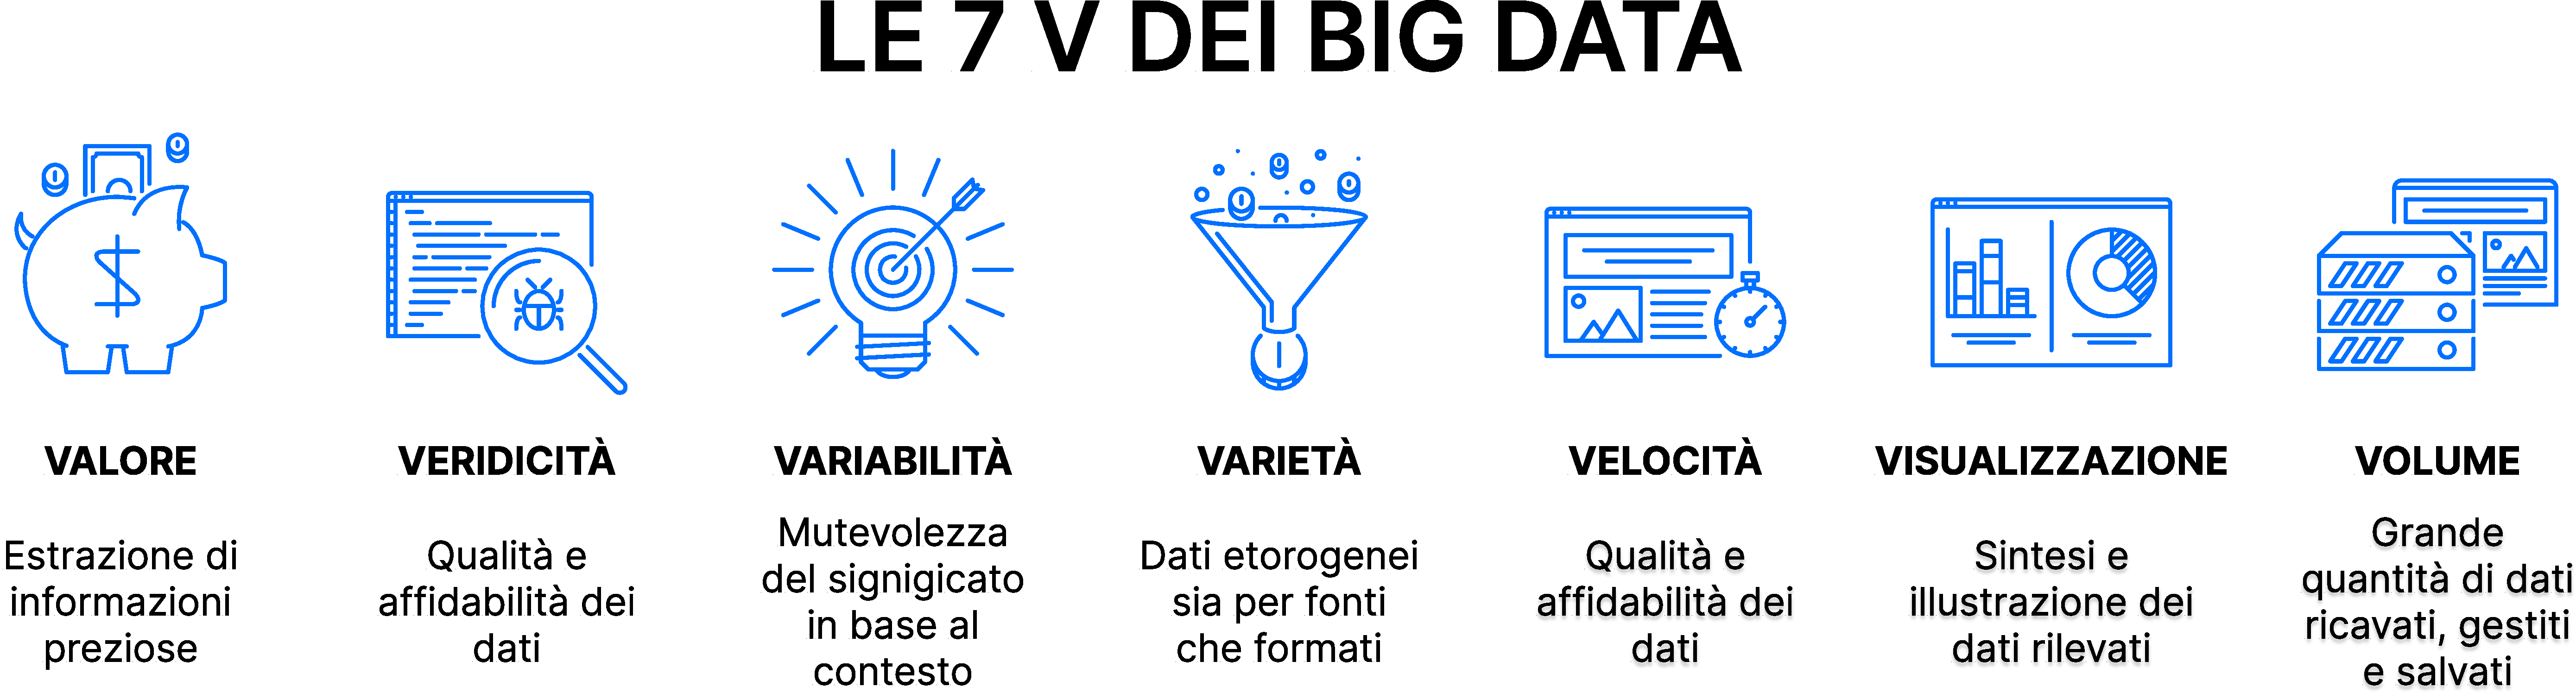
\includegraphics[width=1\linewidth]{figure/capitolo_2/Le 7 V dei Big Data.pdf}
    \caption{Le 7 V dei Big Data}
    \label{fig:Le 7 V dei Big Data}
\end{figure}

\subsection{Strutturazione dei Dati}

Come affermato sopra, una delle caratteristiche dei Big Data è la varietà poiché in un ambiente possibilmente eterogeneo come questo, i dati vengono ricevuti quasi sempre in formati differenti. In base al loro formato, o per meglio dire la loro \textit{struttura}, è necessario adoperare approcci distinti per ottenere le informazioni necessarie.

Quando si parla di \textbf{struttura dei dati} si riferisce ai metodi di organizzazione delle unità di dati all'interno di insiemi più grandi. La creazione e il mantenimento di specifiche strutture di dati aiutano a migliorare l'accesso al valore di quest'ultimi. Man mano che i dati vengono organizzati in modo più elaborato essi diventano più funzionali.

In base alle necessità, all'architettura del progetto e al loro scopo, i dati possono essere salvati in tre diversi modi:

\begin{itemize}
    \item \textbf{Dati strutturati}. I dati strutturati sono dati la cui struttura è predefinita e quindi rispettano tutti la stessa forma prima di essere inseriti all'interno dell'archivio dati. Ciò permette di avere lo stesso insieme di proprietà per i dati che rispettano il medesimo formato. Tali dati vengono anche chiamati dati relazionali poiché è possibile rappresentarli facilmente in un formato tabellare relazionabile tra loro.
    \item \textbf{Dati semi-strutturati}. I dati semi-strutturati sono una tipologia di dati che non è conforme ad una struttura formale di modelli di dati, ma che sfrutta alcuni tipi di tag organizzativi per separare gli elementi semantici che li compongono così da definire delle gerarchie per i campi che contengono le informazioni. Solitamente queste strutture sono adoperate per il salvataggio dei metadati, che contengono delle informazioni strutturate ma non sempre gli stessi campi.
    \item \textbf{Dati non strutturati}. I dati non strutturati sono il tipo di dati che non aderiscono ad uno schema o insieme di regole definito e quindi si presentano in forme o strutture ignote e diverse tra loro. Questo tipo di dati ha una forma sconosciuta e non può essere archiviato in modi tradizionali o analizzato a meno che non vengano trasformati in un formato strutturato. Proprio per questo motivo la gestione di tali dati è un compito impegnativo.
\end{itemize}

Principalmente, i dati contenenti le informazioni vengono salvati in formati strutturati o non strutturati e per questo motivo spesso si incorre nel dubbio sul quale scegliere tra i due formati per il proprio progetto. Di seguito è riportata una tabella che mostra le differenze fra le due tipologie di dati.

\begin{longtable}{|p{2cm}|p{6cm}|p{6cm}|}
    \caption{Differenze tra dati strutturati e non strutturati} \\
    \hline
    \textbf{Ambito di paragone} & \textbf{Dati Strutturati} & \textbf{Dati Non Strutturati} \\
    \hline
    \endfirsthead

    Struttura & I dati strutturati nei Big Data si basano su RDBMS e seguono una struttura a righe-colonne. &  I dati non sono organizzati in un modo definito, per questo motivo non funzionano con alcun set di modelli di dati. \\
    \hline
    Fonti & Provengono principalmente da database relazionali, sistemi di gestione, siti web, applicazioni, dati finanziari, archivi dati, sensori e dispositivi IoT. & Provengono principalmente da file di testo, immagini, video, audio, documenti PDF, e-mail, social media, log e dati di tracciamento, documenti di elaborazione e bot di assistenza.\\
    \hline
    Formati & I loro possibili formati di origini sono: CSV, Excel, DB Relazioni, XML, Parquet ed Avro. & I loro possibili formati di origini sono: TXT, PDF, JPEG, PNG, MP3 e MP4.\\
    \hline
    Modelli & Modello che rispetta una struttura predefinita prima di essere salvati nell'archivio dati. & Sono memorizzati nel proprio formato originale senza essere elaborati finché non eseguiti.\\
    \hline
    Salvataggio & I dati vengono salvati in un formato tabellare e richiedono meno spazio di archiviazione. & Questi dati vengono archiviati come file multimediali o database NoSQL, richiedendo maggiore spazio di archiviazione.\\
    \hline
    Formato & Segue uno schema rigido che fornisce sia coerenza che efficienza. & Non segue una struttura costante e per questo è incoerente.\\
    \hline
    Facilità di analisi & Esistono diversi strumenti di analisi rodati per il recupero, la gestione e l'analisi dei dati. & Gli strumenti per il recupero, la gestione e l'analisi dei dati sono ancora in fase di sviluppo.\\
    \hline
\end{longtable}

In altre parole, analizzando le differenze riportate nella tabella precedente, la scelta di adoperare uno dei due formati di dati dipende da quale sia lo scopo e soprattutto la tipologia di informazioni che si vorrebbero salvare. Non esiste un formato che prevale sull'altro in qualsiasi caso, ma solamente in base alla propria esigenza.

\subsection{Vantaggi e Problematiche dei Big Data}

I Big Data rappresentano il fattore produttivo chiave in un'economia data-driven; molti sono gli ambiti, sia privati che pubblici, in cui l'utilizzo di tecniche di analisi di Big Data ha permesso di creare nuovi servizi, migliorare quelli esistenti, innovare i processi produttivi e distributivi, rendere l'offerta di tutti i prodotti e servizi, migliorare quelli esistenti, innovare i processi produttivi e distributivi, rendere l'offerta di tutti i prodotti e servizi (anche non digitali) più rispondenti alle esigenze dei consumatori e cittadini. Tuttavia, benché stimolante, l'analisi dei Big Data è un'operazione complessa. I data scientist si occupano dell'analisi dei dati per offrire all'azienda informazioni e raccomandazioni utili e i data engineer sono responsabili di identificare, assemblare e gestire gli strumenti necessari in un flusso di dati. Ogni singola fase rappresenta delle sfide in termini di integrazione, capacità di storage e riduzione dei budget IT\footnote{\textit{URL Fonte}: www.redhat.com/en/topics/big-data}.

Pertanto di seguito sono riportate alcune delle problematiche da considerare se si ha l'intenzione di predisporre un sistema per l'applicazione dei Big Data\footnote{\textit{URL Fonte}:https://tinyurl.com/yv7nwc4d}:

\begin{itemize}
    \item \textit{Organizzazione e accessibilità dei dati}. La principale problematica associata ai Big Data consiste nel capire come gestire il volume di informazioni ottenute affinché pervengano correttamente nelle applicazioni.
    \item \textit{Controllo qualità}. Garantire l'accuratezza e la qualità dei dati può essere difficile e dispendioso in termini di tempo, soprattutto quando tali dati arrivano rapidamente e a volumi molto elevati. Prima di effettuare qualsiasi analisi, occorre assicurarsi che i processi di raccolta, elaborazione e pulizia dei dati siano integrati, standardizzati e ottimizzati.
    \item \textit{Sicurezza dei dati}. Con l'aumento delle violazioni di dati, la protezione di quest'ultimi ha sempre più importanza. Così come il sistema di analisi cresce, aumenta anche la possibilità di riscontrare problemi di sicurezza sotto forma di dati fittizi, fughe di informazioni, problematiche relative alla conformità e alla vulnerabilità del software. Per ridurre alcune di tali preoccupazioni, occorre crittografare i dati e condurre regolarmente controlli di sicurezza.
    \item \textit{Scelta degli strumenti giusti}. Dover scegliere tra i tantissimi strumenti e tecnologie disponibili può creare confusione. Ecco perché è importante provvedere alla formazione, rimanere sempre aggiornati e, se possibile, assumere o consultare uno specialista ove necessario.
\end{itemize}

Una volta mostrate le problematiche a cui fare attenzione per sviluppare un sistema di gestione dei Big Data, è ora importante mostrare quanto siano rilevanti i vantaggi nell'intraprendere questa scelta\footnote{\textit{URL Fonte}: www.oracle.com/big-data/what-is-big-data}.

\begin{itemize}
    \item \textit{Sviluppo di prodotti e servizi}. L'analisi dei Big Data consente agli sviluppatori di prodotti di analizzare dati non strutturati, quali le recensioni dei clienti e le tendenze culturali, e di reagire prontamente anche predicendo le eventuali richieste anticipando la domanda della propria utenza.
    \item \textit{Manutenzione predittiva}. I fattori che possono prevedere guasti meccanici possono essere nascosti tra i dati strutturati, riguardanti le informazioni della strumentazione, oppure nei dati non strutturati, riguardanti le informazioni generate da tali dispositivi. Analizzando queste indicazioni di potenziali problemi prima che si verifichino, le aziende possono svolgere la manutenzione in modo più efficiente in termini di costi e tempistiche.
    \item \textit{Customer Experience}. I Big Data consentono di raccogliere dati da social media, visite sui siti web, registri delle chiamate e altre fonti allo scopo di migliorare l'esperienza di interazione tra l'utente e l'azienda. In altre parole, l'analisi di tali dati permette alle organizzazioni di migliorare l'esperienza vissuta dai clienti con il loro brand in modo da ottenere una maggiore soddisfazione da parte dell'utente, che corrisponde a possibili nuovi introiti.
    \item \textit{Frode e conformità}. Gli scenari di sicurezza e i requisiti di conformità sono in continua evoluzione. I Big Data aiutano a identificare i modelli nei dati che indicano frodi e ad aggregare grandi volumi di informazioni per rendere i rapporti normativi molto più veloci. Gli insight generati dall'analisi dei tali dati consentono alle aziende di anticipare il rischio e a prepararsi ad eventuali malevoli imprevisti.
    \item \textit{Efficienza operativa}. L'efficienza operativa potrebbe non essere sempre un argomento innovativo, ma ha molta rilevanza nel mondo dei Big Data. In tale ambito, è possibile analizzare e valutare la produzione, i feedback e i resi da parte dei clienti, e ulteriori fattori per ridurre le interruzioni e anticipare le future richieste. I Big Data possono essere utilizzati anche per migliorare il processo decisionale in linea con l'attuale domanda di mercato.
    \item \textit{Incentivare l'innovazione}. I Big Data possono aiutare ad innovare studiando le interdipendenze tra essere umani, istituzioni, entità e processi e quindi determinando nuovi modi per utilizzare tali insight. Sfruttare gli insight così generati crea infinite possibilità, dal migliorare le decisioni su considerazioni interne a fornire nuovi prodotti e servizi.
\end{itemize}

\subsection{Thick Data}

Come abbiamo potuto comprendere, i Big Data non riescono a mostrare tutte le informazioni che si potrebbero recuperare da una determinata fonte. Per questo motivo, esiste un'altra famiglia di dati che ha la sua rilevanza nel mondo dell'analisi dei dati, ovvero i \textit{thick data}.

I \textbf{thick data} riguardano le informazioni sul significato e le connessioni che le persone attribuiscono ai servizi o alle tecnologie, così come il processo con cui li consumano. L'idea alla base è che l'analisi interpretativa dei dati deve seguire un approccio non solamente quantitativo ma anche qualitativo puntando a ulteriori fattori come quelli esterni ai dati a disposizione. Di seguito è riportata una tabella che permette di comprendere la differenza tra i Big Data ed i thick data \cite{big_data_and_thick_data}.

\begin{longtable}{|p{4cm}|p{5cm}|p{5cm}|}
    \caption{Differenze tra dati strutturati e non strutturati} \\
    \hline
    \textbf{Caratteristiche} & \textbf{Big Data} & \textbf{Thick Data} \\
    \hline
    \endfirsthead 
    
    Formato & Dati in formato numerico. & Dati non numerici, qualitativi formato. \\ 
    \hline
    Volume & Solitamente quantità elevate. & Solitamente quantità basse. \\ 
    \hline
    Metodi di collezione & Documenti digitali, archivio digitalizzato record, streaming di dati, log di trasmissione, dati numerici recuperati da Internet. & Osservazioni e interviste dirette ai partecipanti, focus group, sondaggi a risposta aperta, video registrazioni, dati qualitativi provenienti da Internet \\ 
    \hline
    Analisi & Ricerche di scienziati sociali e computazionali. & Ricerche di antropologi e etnografi. \\ 
    \hline
    Requisito di immersione & Non è necessario che gli analisti siano in loco per analizzare i dati. & Di solito in loco o con l'osservazione diretta online, e immersi nel contesto. \\ 
    \hline
    Ruolo nella soluzione dei problemi & Generare soluzioni a problemi in gran parte noti, generando decisioni automatiche. & Identifica i problemi che contano di più per le parti interessate e testa le soluzioni prima di espanderle. \\ 
    \hline
    Punti di forza & \textit{Scala}: generare insight generalizzabili a un'ampia porzione o a un'intera popolazione. & \textit{Profondità}: identificare ciò che interessa in primo luogo agli stakeholder; dipingere un quadro olistico di determinate esperienze. \\ 
    \hline
\end{longtable}


In altre parole, i thick data, analizzando il contesto in cui i dati vengono recuperati, permettono di comprendere le motivazioni che hanno portato le persone a svolgere determinate scelte, ciò permette anche di comprendere quali sono stati i ragionamenti e le sensazioni che hanno portato a prendere una determinata decisione da parte di un utente. Di conseguenza, quando i Big Data vengono combinati con i thick data, è possibile generare un quadro più completo delle esigenze, dei requisiti e delle preferenze dei consumatori.

\begin{figure}[H]
    \centering
    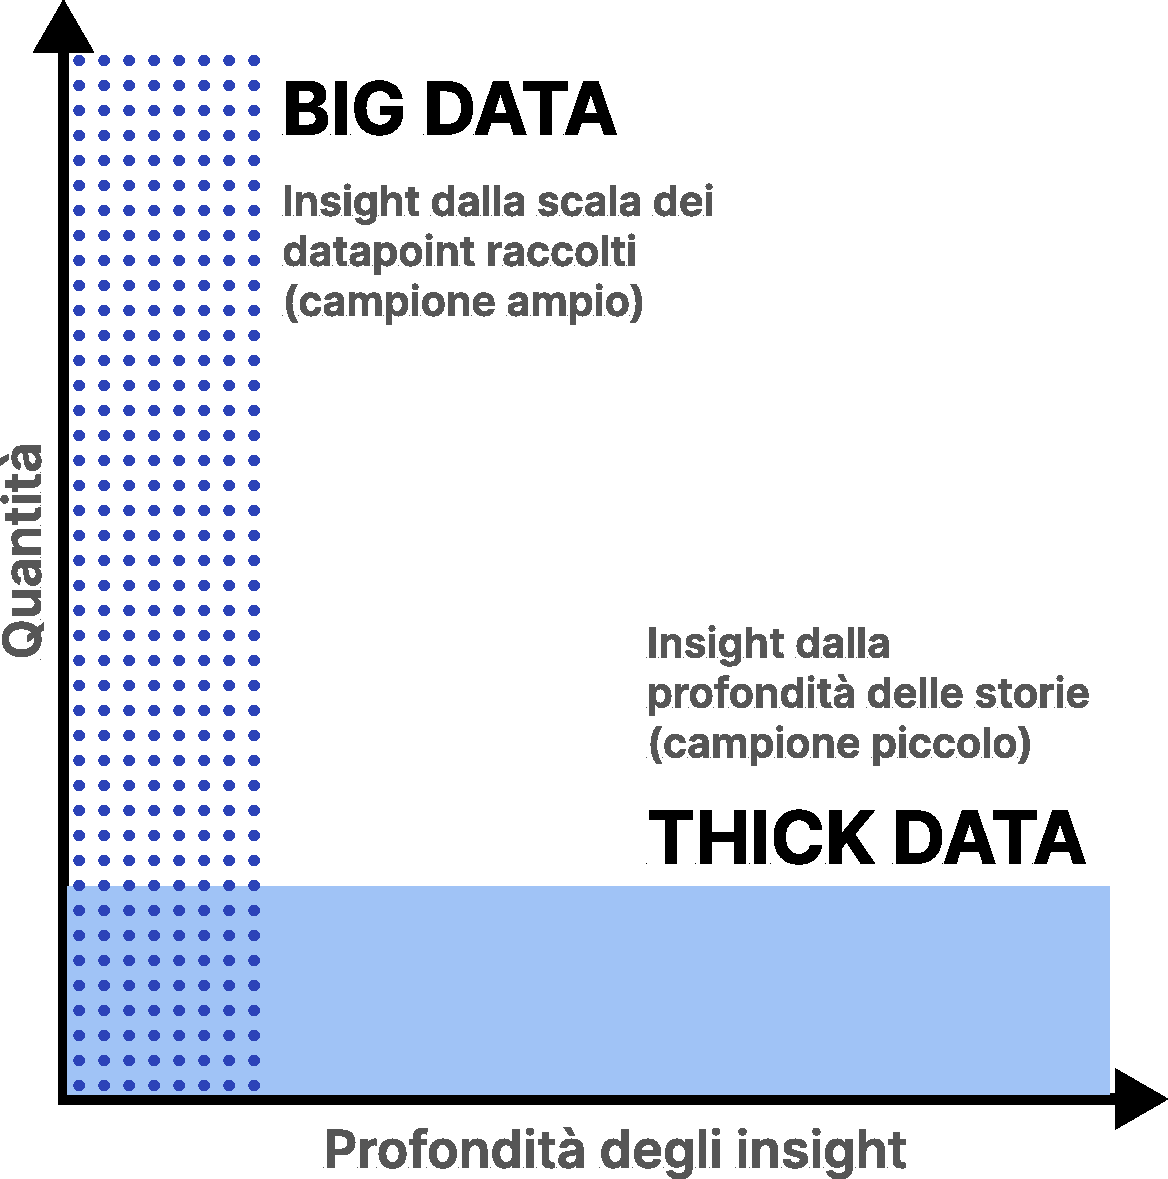
\includegraphics[width=0.4\linewidth]{figure/capitolo_2/Thick and Big Data.pdf}
    \caption{Schema dei Thick e Big Data}
    \label{fig:Thick and Big Data}
\end{figure}

\subsection{Differenza Tra i Big Data e i Dati Tradizionali}

Di seguito è riportata una tabella che permette di descrivere le differenze tra i Big Data e i dati tradizionali\footnote{\textit{URL Fonte}: https://tinyurl.com/2hwcr5ms}.

\begin{longtable}{|p{4cm}|p{5cm}|p{5cm}|}
    \caption{Differenza tra Big Data e dati tradizionali} \\
    \hline
    \textbf{Caratteristica} & \textbf{Big Data} & \textbf{Dati tradizionali} \\
    \hline
    \endfirsthead 
        Dimensioni & Volumi approssimativamente misurati in petabyte, exabyte o zettabyte & Volumi approssimativamente misurati in gigabyte e terabyte\\
        \hline
        Organizzazione & Dati, principalmente, grezzi o non strutturati con schemi dinamici & Dati strutturati organizzati in record, file e tabelle, solitamente sono dati relazionali\\
        \hline
        Architettura & Quasi sempre gestiti adoperando sistemi distribuiti dato il volume e la complessità & Solitamente gestiti adoperando sistemi con strutture centralizzate\\
        \hline
        Fonti & Derivano da fonti di qualsiasi genere: programmi, social media, dispositivi IoT, ecc. & Derivano in genere da determinati programmi con uno scopo specifico\\
        \hline
        Analisi & L'analisi può essere svolta sia in modo incrementale che in tempo reale & Analisi incrementale: si verifica un evento, i dati vengono generati, gestiti e poi analizzati\\
        \hline
\end{longtable}

I Big Data e i dati tradizionali hanno scopi diversi ma correlati, che ben possono collaborare tra loro.

\section{I Data Warehouse}

Il \textit{data warehousing} ha iniziato il proprio percorso negli anni '70 grazie a William H. Inmon e Ralph Kimball poiché ritenevano che i database basati sui modelli, per quanto efficienti nel trattamento dei dati relazionali, non lo fossero altrettanto per casi di report analitici complessi. Le aziende necessitavano di un'analisi dei dati migliore per prendere decisioni aziendali efficaci e ben ragionate. Ai tempi non esisteva una metodologia di integrazione adeguata disponibile per rappresentare i dati necessari che le compagnie immagazzinavano nei vari sistemi di supporto \cite{researchgate_data_warehouse}.
Per sopperire a tali necessità Inmon e Kimball condussero una ricerca dettagliata sui \textit{sistemi di supporto decisionale} e sui \textit{data warehouse}, sviluppando un loro approccio nella creazione di tali sistemi che permettessero attività di analisi, centralizzando grandi quantità di dati derivanti da più origini e formati.

\subsection{Definizione}

Il padre del termine \textbf{data warehouse} è William H. Inmon che, nel finire degli anni '90, lo definì come «una raccolta di dati orientati al soggetto, integrati, non volatili e varianti nel tempo, finalizzata a supportare le decisioni della direzione aziendale». In quest'ottica, i data warehouse assumono un doppio scopo nella gestione dei dati \cite{inmon_building_the_data_warehouse}:

\begin{itemize}
    \item Possibilità di essere interrogati per recuperare specifiche informazioni necessarie nell'immediato.
    \item Mantenimento dei dati con l'obiettivo di sfruttarli in futuro quando avranno assunto maggior valore.
\end{itemize}

Analizzando meglio la suddetta definizione di Inmon, è possibile affermare che essa si basi su quattro caratteristiche fondamentali che riguardano i dati di cui un data warehouse si compone. Per avere una migliore comprensione del concetto, di seguito sono riportate le spiegazioni di tali caratteristiche \cite{researchgate_data_warehouse_architecture}:

\begin{enumerate}
    \item \textit{Orientati al soggetto}: tutti i dati relativi a un determinato argomento vengono raccolti e archiviati come un unico insieme in un formato utile; tali dati vengono presentati in base a soggetti specifici oppure aree di interesse.
    \item \textit{Integrati}: i dati vengono archiviati in modo globalmente accettabile, ovvero rispettando una determinata convenzione cosicché le loro strutture e attributi possano essere coerenti anche indipendentemente dal caso in cui il loro formato originale di archiviazione, dovuto a sistemi operativi eterogenei, siano differenti o addirittura incompatibili.
    \item \textit{Non volatili}: le informazioni ricavabili dai dati non devono cambiare ad ogni esecuzione di un processo di recupero o analisi; tali informazioni sono coerenti indipendentemente dal momento in cui vengono richieste al data warehouse.
    \item \textit{Varianti nel tempo}: questa caratteristica, per quanto a primo impatto possa sembrare in contraddizione con la precedente, in realtà la avvalora. Quando si parla di “varianti nel tempo” si intende che le informazioni recuperate possano variare dipendentemente dal periodo in cui vengono recuperate e ciò permette di mantenere una traccia dei cambiamenti avvenuti così che possano descrivere la storia del soggetto a cui si fa riferimento. Ciò naturalmente è possibile inserendo il periodo di riferimento all'interno delle informazioni registrate nei dati salvati e salvando tutti gli stati che li contraddistinguono.
\end{enumerate}

\subsection{Obiettivi dei Data Warehouse}
Per comprendere meglio cosa sono i data warehouse è utile fare una ricapitolazione di quali sono gli obiettivi per cui vengono utilizzati \cite{kimball_the_data_warehouse_toolkit}.

\begin{itemize}
    \item \textit{Rendere le informazioni facilmente accessibili}. I dati devono essere intuitivi e ovvi per l'analista e non solo per lo sviluppatore. Le strutture e le etichette dei dati dovrebbero rappresentare i processi mentali e il vocabolario dell'azienda. 
    \item \textit{Presentare le informazioni in modo coerente}. I dati devono essere attentamente raccolti da una varietà di fonti, puliti, sottoposti a controlli di qualità e resi disponibili solo quando adatti all'uso da parte degli utenti preposti.
    \item \textit{Il sistema deve adattarsi ai cambiamenti}. Le esigenze degli utenti, le condizioni aziendali, i dati e la tecnologia sono tutti soggetti a cambiamenti. Il sistema DW deve essere progettato per gestire cambiamenti inevitabili in modo delicato, tale da non invalidare i dati o le applicazioni esistenti. Se i dati descrittivi nel sistema devono essere modificati, è necessario tener conto in modo appropriato delle modifiche e rendere queste modifiche trasparenti agli utenti.
    \item \textit{Presentare le informazioni tempestivamente}. Venendo adoperato in modo sempre più intensivo per le decisioni operative, i dati grezzi possono dover essere convertiti in informazioni utilizzabili entro ore, minuti o addirittura secondi.
    \item \textit{Proteggere i “beni informativi”}. Le informazioni più preziose di un'azienda sono solitamente conservate nei data warehouse. Proprio per questo motivo tali sistemi devono controllare efficacemente l'accesso alle informazioni confidenziali della compagnia.
    \item \textit{Il sistema deve essere affidabile per migliorare i processi decisionali}. I dati presenti all'interno del sistema devono essere sicuri e appropriati per supportare le eventuali decisioni prese dall'azienda. Il processo decisionale di una compagnia viene solitamente avvalorato dall'analisi dei dati rispetto all'ambito della scelta e per questo motivo i dati in esso contenuti devono essere corretti e coerenti.
\end{itemize}

\subsection{Tipologia di Dati}

È possibile identificare in tre principali categorie i dati che alimentano un sistema di data warehouse \cite{vercellis_business_intelligence}:
\begin{itemize}
    \item \textbf{Dati interni}. Sono principalmente archiviati nei database, denominati \textit{sistemi transazionali} o \textit{operativi}, che corrispondono ai punti cardine di un sistema informativo aziendale. I dati interni vengono raccolti attraverso applicazioni transazionali che supervisionano regolarmente le operazioni di un'azienda. Questa collezione di applicazioni software transazionali è chiamata \textit{Enterprise Resource Planning (ERP)}. Questi dati, fondamentali per l'analisi e i reporting aziendali, provengono solitamente da diverse componenti del sistema informativo:
        \begin{itemize}
            \item \textit{Sistemi back-office}: raccolgono record transazionali derivanti dalle azioni/attività svolte dai software;
            \item \textit{Sistemi front-office}: raccolgono dati derivanti dalle attività svolte per rapportarsi con gli utenti finali;
            \item \textit{Sistemi web-based}: raccolgono dati creati dalle interazioni dei sistemi con i clienti che li utilizzano.
        \end{itemize}
    \item \textbf{Dati esterni}. Esistono diverse fonti di dati esterni che possono essere utilizzate per arricchire il valore delle informazioni archiviate nei database interni. Ad esempio, è possibile fare riferimento ad alcune agenzie che raccolgono e mettono a disposizione dati relativi alle vendite, alla quota di mercato e alle previsioni future per specifici settori industriali, nonché economici e finanziari. 
    \item \textbf{Dati personali}. Solitamente gli analisti e i decision maker che svolgono ricerche aziendali si affidano anche ad informazioni e valutazioni personali archiviate all'interno di fogli di lavoro o database locali situati nei propri computer. Il recupero di tali informazioni e la loro relativa integrazione con i dati strutturati provenienti sia da fonti interne che esterne è uno degli obiettivi dei \textit{sistemi di gestione delle informazioni} (\textit{Knowledge Managament Systems, KMS}).
\end{itemize}

\subsection{La Modellazione dei Dati}
Esistono molte tecnologie di database e strumenti per l'elaborazione dei dati, inoltre, insiemi di dati differenti richiedono strumenti ad hoc per far sì che le analisi svolte possano reputarsi efficaci. La creazione di \textit{modelli di dati}, o \textit{modellazione di dati}, offre la possibilità di comprendere i dati che bisogna gestire e prendere le giuste decisioni a riguardo.
La \textbf{modellazione dei dati} è un processo adoperato per analizzare e definire tutti i diversi tipi di dati che l'azienda gestisce (raccoglie o produce) che siano di supporto a processi aziendali nel relativo ambito di competenza. Poiché sono le compagnie a determinare il modo ed il momento dell'applicazione di tali dati, il processo di modellazione di quest'ultimi è un importante esercizio utile a comprendere e chiarire quali sono i requisiti a loro associati\footnote{\textit{URL Fonte}: https://powerbi.microsoft.com/en-us/what-is-data-modeling/}.

\subsubsection{Categorie dei Modelli di Dati}

Esistono tre categorie principali che rappresentano i livelli di pensiero durante lo sviluppo di un modello di dati, esse si dividono dipendentemente dal loro grado di astrazione, ovvero\footnote{\textit{URL Fonte}: https://www.ibm.com/topics/data-modeling}:

\begin{itemize}
    \item \textit{Modelli di dati concettuali}. Anche denominati modelli di dominio, offrono una visione d'insieme di ciò che il sistema andrà a contenere, come esso sarà organizzato e quali regole di business saranno adoperate. Tali modelli sono di solito creati durante il processo di raccolta dei requisiti iniziali del processo. In genere includono le classi di entità, le loro caratteristiche ed i relativi vincoli, le relazioni tra loro e i requisiti di sicurezza ed integrità dei dati associati.
    \item \textit{Modelli di dati logici}. Sono meno astratti e forniscono maggiori dettagli sui concetti e le relazioni rispetto al dominio in esame, o in altre parole il flusso dei dati e il contenuto del database. Si esegue uno dei vari sistemi di notazione formale per la modellazione dei dati. Tali modelli indicano gli attributi dei dati e mostrano le relazioni tra le entità. I modelli di dati logici sono utili in ambienti di implementazione altamente procedurali o in caso di progetti orientati intrinsecamente ai dati.
    \item \textit{Modelli di dati fisici}. Questi modelli forniscono uno schema di come i dati saranno fisicamente immagazzinati in un database definendo le specifiche delle modalità di realizzazione del modello logico. Tali modelli, come è facile dedurre, sono i meno astratti tra le tre tipologie. Offrono un design finalizzato che può essere implementato come un database relazionale, includendo tabelle associative che illustrano le relazioni tra le entità.
\end{itemize}

\subsubsection{Tipologie di Modellazione}

Più precisamente, il tipo di modellazione dei dati definisce la struttura logica di quest'ultimi, ovvero il modo in cui essi vengono archiviati logicamente, comportando anche la definizione delle modalità di archiviazione, organizzazione e recupero. Le principali tipologie sono tre, ovvero\footnote{\textit{URL Fonte}: https://tinyurl.com/nrypx7nj}:

\begin{itemize}
    \item \textbf{Relazionale}. È il modello di database maggiormente in uso, esso archivia i dati in record di formato fisso e li organizza in tabelle strutturate in righe e colonne. Il fattore più importante di questa tipologia di database sono naturalmente le relazioni definite all'interno di tale struttura, il cui compito è di creare un legame tra due dati comuni (detti chiavi) che permettono di collegare due tabelle tra loro. Il tipo di modello di dati più semplice presenta due elementi in cui i dati grezzi vengono suddivisi in “misure” (i valori numeri adoperati nei calcoli matematici) e “dimensioni” (valori numerici o testuali che danno informazioni secondarie non adoperabili per dei calcoli).
    \item \textbf{Dimensionale}. È un approccio meno rigido e strutturato che favorisce una struttura di dati contestuale rispetto all'ambito di utilizzo o all'ambiente aziendale. Gli elementi fondamentali di questa struttura di database sono definiti “fatti” (i dati primari) e sono accompagnate da informazioni di riferimento definite “dimensioni” (i dati associativi). Il recupero dei dati può essere rapido ed efficiente, ma la mancanza di collegamenti relazioni può rendere tale processo più complicato. 
    \item \textbf{Entità-Relazione}. È un approccio che sfrutta il modello E-R (Entità-Relazione) con una struttura di dati aziendali in formato grafico contenete caselle di varie forme che rappresentano attività o funzioni (entità) e righe che rappresentano associazioni e dipendenze (relazioni). Tale modello viene adoperato per creare database relazioni in cui ogni riga rappresenta un'entità e i campi in quella riga contengono degli attributi.
\end{itemize}


\subsection{Il Modello Multidimensionale dei Dati}

Secondo diversi studi è emerso che i modelli di dati tradizionali, come il modello E-R e il modello relazionale, non forniscono un buon supporto ai sistemi appositi per la gestione di dati a fini analitici. Per sopperire a tale problematica, nel tempo sono emersi differenti modelli dai dati basati su una visione multidimensionale dei dati in questione. Questi modelli multidimensionali categorizzano i dati come \textit{fatti} (anche definiti come “misure”) o \textit{dimensioni} \cite{ieee_multidimensional_data_modeling}.

Il \textbf{modello multidimensionale} deriva la sua idea dalla constatazione che gli oggetti che influenzano il processo decisionale sono \textit{fatti} che accadono nel mondo aziendale ed ogni occorrenza di un fatto corrisponde ad un evento accaduto. Inoltre, per ognuno dei fatti registrati si è interessati ai valori di insiemi di \textit{misure} o \textit{metriche} che descrivono quantitativamente gli eventi in questione. Poiché gli eventi da registrare sono moltissimi, viene adoperato un modello che permette di selezionarli e raggrupparli come se fossero collocati all'interno di uno spazio n-dimensionale i cui assi, definiti come \textit{dimensioni} di analisi, determinano diverse prospettive per la loro identificazione \cite{unibo_introduzione_al_data_warehousing}.

\subsubsection{Il Cubo Multidimensionale}

I database che sfruttano il modello multidimensionale considerano i dati come cubi che generalizzano i fogli di calcolo a qualsiasi numero di dimensioni. Inoltre, i cubi supportano gerarchie nelle dimensioni e misure senza duplicare le loro definizioni. Una raccolta di cubi correlati costituisce un database multidimensionale oppure un data warehouse. Sebbene l'immagine associabile all'idea del cubo sia di sole tre dimensioni, in realtà un cubo può teoricamente avere un numero indefinito di dimensioni, per quanto l'aumentare di dimensioni comporti la necessità di sistemi appositi per poterli gestire \cite{researchgate_multidimensional_db}.

Più precisamente, in un cubo le dimensioni definiscono la struttura del cubo utilizzata per effettuare le sezioni che lo compongono, mentre le misure forniscono valori numerici aggregati che siano utili all'utente finale -- come rappresentato nella Figura \ref{fig:Multidimensional Data Cube}\footnote{\textit{URL Figura}: https://tinyurl.com/4su6hx66}--. Un cubo consente ad un'applicazione di recuperare i valori delle misure come se queste si trovassero nelle celle del cubo, dove quest'ultime vengono definite per ogni possibile valore riepilogativo. In altre parole, una cella è definita dall'intersezione degli elementi sull'asse delle dimensioni e contiene i valori aggregati delle misure che corrispondono a quella specifica intersezione\footnote{\textit{URL Fonte}: https://tinyurl.com/999wwy8r}.

\begin{figure}
    \centering
    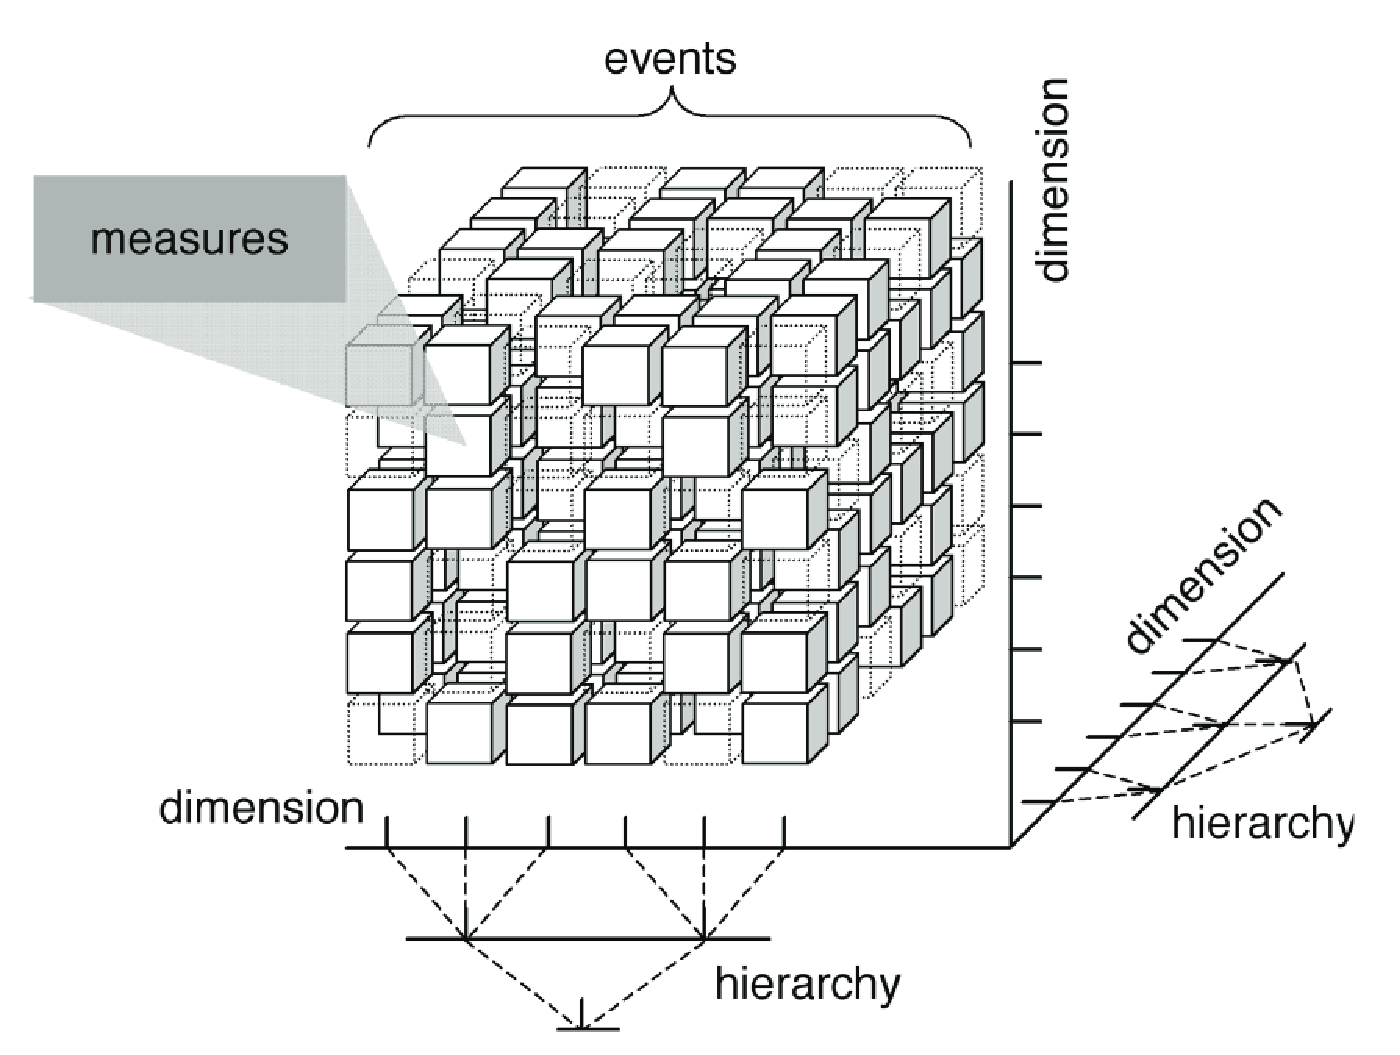
\includegraphics[width=0.75\linewidth]{figure/capitolo_2/Multidimensional Data Cube.pdf}
    \caption{Rappresentazione di dati Multidimensionali sottoforma di cubo}
    \label{fig:Multidimensional Data Cube}
\end{figure}

Per semplificare il concetto, una tabella di un database è strutturata come un foglio di calcolo e memorizza i singoli record in un formato bidimensionale, riga per colonna; ogni fatto corrisponde all'intersezione di due dimensioni, una riga e una colonna. Invece, un cubo multidimensionale estende la singola tabella con livelli ulteriori aggiungendo una dimensione per ogni livello permettendo di rappresentare in questo modo maggiori informazioni per un singolo evento.

\subsection{Database OLTP e OLAP}

I database relazionali sono stati uno dei punti cardine delle infrastrutture delle applicazioni aziendali per più di venti anni. Con l'avanzare della tecnologia si pose l'obiettivo di fornire alle compagnie un sistema di gestione delle informazioni che coprisse tutti gli ambiti principali che vanno dalla pianificazione dei processi aziendali fino alle analisi individuali; tuttavia, ciò non è stato possibile. Più complessi diventano i requisiti aziendali e maggiore è stato il focus sul migliorare l'elaborazione transazionale, creando appositi database che prendono il nome di sistemi \textbf{OLTP} (\textit{On-Line Transactional Processing}, o ``elaborazione transazionale on-line''). Ciò ha comportato la necessità di spostare le applicazioni di ambito analitico e finanziario in sistemi separati ad hoc che avessero maggiore flessibilità e prestazioni, prendendo il nome di sistemi \textbf{OLAP} (\textit{On-Line Analytical Processing}, o ``elaborazione analitica on-line''). Entrambi i sistemi sono basati sulla teoria relazionale dei dati, ma utilizzano approcci tecnici differenti. Inoltre, l'OLTP è il prerequisito necessario per l'OLAP, ma solo con l'OLAP le aziende possono comprendere al meglio i dati generati dal proprio lavoro e trarre delle conclusioni che permettano di migliorarlo \cite{scribd_oltp_olap}.

I sistemi OLTP sono strutture progettate per alti volumi di query con accesso specifico con l'obiettivo di massimizzare l'efficienza di queste operazioni, mentre i sistemi OLAP utilizzano tecnologie di archiviazione dei dati per supportare l'analisi e l'estrazione di dati storici a lungo termine per fornire agli analisti dei report da cui ricavare informazioni per prendere decisioni aziendali \cite{ieee_oltp_olap}.
Per comprendere meglio questo discorso, di seguito vengono spiegati i concetti di OLAP e OLTP, in modo da poter approfondire l'argomento.

\begin{itemize}
    \item \textit{OLTP}. Questi database in genere comprendono dati transazionali, ovvero informazioni che tengono traccia delle informazioni correlate alle attività di un'azienda. Gli stati che descrivono le transazioni dei dati devono però essere atomiche\footnote{Un'operazione si definisce \textit{atomica} se questa ha sempre un esito o positivo o negativo, non può rimanere in uno stato parziale.} e coerenti. Tali sistemi sono progettati per elaborare e archiviare in modo efficiente singole transazioni, permettendo in questo modo di gestire grandi quantità di transazioni in modo indipendente\footnote{\textit{URL Fonte}: https://tinyurl.com/mr3j5y8c}.
    \item \textit{OLAP}. È una tecnologia che consente di organizzare i database aziendali di grandi dimensioni e supporta l'esecuzione di analisi complesse. Può essere usata per seguire query di analisi complesse senza influire negativamente sulle attività dei sistemi transazionali. Poiché i database utilizzati dalle aziende, principalmente OLTP, non sono progettati per sopperire a necessità di analisi, il recupero delle informazioni da questi sistemi è un compito esoso sia in termini di tempo che di prestazioni. A questo scopo sono stati ideati i database OLAP, ottimizzati appositamente per gestire intensi carichi di lavoro in lettura e ridotti in scrittura\footnote{\textit{URL Fonte}: https://tinyurl.com/3kp65m6v}.
\end{itemize}

Di seguito è riportata una tabella riepilogativa che spiega le differenze tra un database OLAP e uno OLTP\footnote{\textit{URL Fonte}: https://aws.amazon.com/compare/the-difference-between-olap-and-oltp/}.

\begin{longtable}{|p{4cm}|p{5cm}|p{5cm}|}
    \caption{Differenze tra database OLTP e OLAP}
    \label{tab:oltp_vs_olap}\\
    \hline
    \textbf{Criteri} & \textbf{OLAP} & \textbf{OLTP}\\
    \hline
    \endfirsthead 
        Scopo & Aiuta ad analizzare grandi volumi di dati per supportare il processo decisionale. & Consente di gestire ed elaborare transazioni in tempo reale.\\
        \hline
        Origine dati & Utilizza dati storici e aggregati provenienti da diverse origini. & Utilizza transazioni in tempo reale provenienti da un'unica origine.\\
        \hline
        Struttura dei dati & Adopera database multidimensionali (cubi) oppure database relazionali. & Adopera solo database relazioni.\\
        \hline
        Modello dei dati & Utilizza lo schema a stella, a fiocco di neve oppure altri modelli analitici. & Utilizza modelli normalizzati o denormalizzati.\\
        \hline
        Volume dei dati & Ha requisiti di archiviazione elevati (TB o PB). & Ha requisiti di archiviazione inferiori (GB).\\
        \hline
        Tempo di risposta & Ha tempi di risposta più lunghi (s o m). & Tempi di risposta brevi (ms).\\
    \hline
    
\end{longtable}

\subsection{Componenti dei Data Warehouse}
Il processo di data warehousing viene definito dalla piattaforma Corporate Finance Institute come «il processo di raccolta e archiviazione dei dati da varie fonti e dalla loro gestione per fornire preziose intuizioni aziendali. Il data warehousing è una combinazione di tecnologia e componenti che consentono un utilizzo strategico dei dati»\footnote{\textit{URL Fonte}: https://tinyurl.com/4m8zde4d}. Per comprendere al meglio come funziona, sarebbe utile analizzare quali sono i componenti -- riportati nella Figura \ref{fig:Data Warehouse Components} -- che definiscono la struttura dei data warehouse\footnote{\textit{URL Fonte}: https://www.altexsoft.com/blog/enterprise-data-warehouse-concepts/}:

\begin{itemize}
    \item \textbf{Fonti di dati}. Queste rappresentano tutte le origini da cui i dati recuperati in un formato grezzo.
    \item \textbf{Livello di ingestione}. Tale livello rappresenta il componente atto al recupero dei dati che andranno a comporre un data warehouse. Per eseguire tale compito esiste il cosiddetto \textit{processo ETL} (\textit{Extract, Transform, Load}). Tale procedura consiste nel connettersi alle fonti di dati per estrarre, trasformare e caricare i dati grezzi in un sistema di archiviazione centralizzato.
    \item \textbf{Staging Area (opzionale)}. Corrisponde ad un'area di archiviazione intermedia, utilizzata dagli strumenti di ETL per eseguire le operazioni di elaborazione prima che i dati vengano effettivamente caricati all'interno del data warehouse. In altre parole, è il punto in cui i dati vengono ripuliti, deduplicati, suddivisi, uniti e convertiti in un formato unificato per adattarsi al modello da adoperare, precedentemente definito, all'interno del DW. 
    \item \textbf{Livello di archiviazione}. Corrisponde allo spazio di archiviazione dove i dati vengono caricati.
    \item \textbf{Modulo dei metadati}. Tutti i metadati relativi ai dati recuperati, sono archiviati in questo apposito modulo e sono gestiti da un manager predisposto. In alcuni casi, potrebbe essere presente uno strato aggiuntivo costruito sopra l'intera infrastruttura per curare i metadati. 
    \item \textbf{Data mart (opzionale)}. In alcuni casi, un DW può essere un insieme di sottosezioni più piccole chiamate \textit{data mart}, costituite da dati riguardanti ognuno un determinato ambito di riferimento.
    \item \textbf{Livello di presentazione}. Il blocco finale di un data warehouse, ma non per importanza, riguarda gli strumenti che forniscono un accesso semplificato e diretto ai dati per gli utenti finali. Questo livello serve come interfaccia per la visualizzazione dei dati, la generazione di report aziendali e l'estrazione di informazioni separate per specifici compiti.
\end{itemize}

\begin{figure}[H]
    \centering
    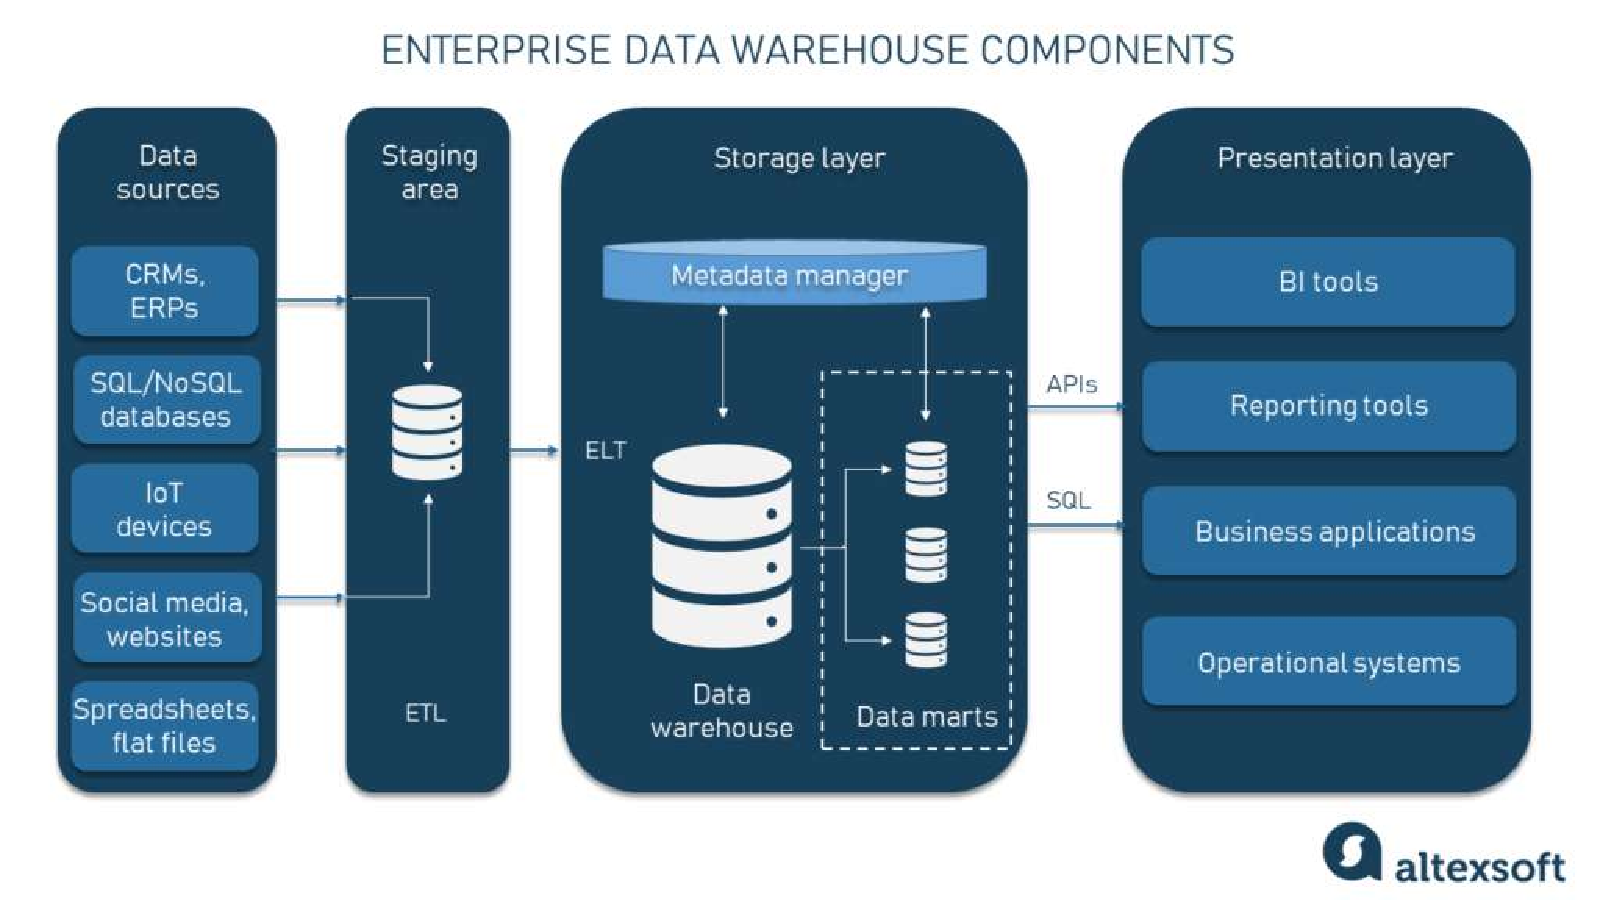
\includegraphics[width=0.75\linewidth]{figure/capitolo_2/Data Warehouse Components.pdf}
    \caption{Componenti di un Data Warehouse}
    \label{fig:Data Warehouse Components}
\end{figure}

\subsection{Architettura dei Data Warehouse}

I data warehouse non sono sistemi semplici. La loro complessità intrinseca, derivata dalla tipologia di problemi che sono destinati a risolvere, ovvero fornire agli analisti una visione unificata e facilmente leggibile delle informazioni, si aggiunge alla mancanza di un preciso modello che permetta di definire quali tecniche o approcci debbano essere applicati e quale sia il metodo per lo sviluppo di tali sistemi \cite{kelly_data_warehousing_in_action}.

Durante gli anni sono state sviluppate diverse architetture per la creazione di un sistema di data warehousing, principalmente possono essere suddivise in tre tipologie\footnote{\textit{URL Fonte}: https://www.interviewbit.com/blog/data-warehouse-architecture/}:

\begin{itemize}
    \item \textbf{Architetture a singolo livello}. Sono utilizzate per l'elaborazione di dati batch e in tempo reale. I dati vengono prima trasferiti ad un'architettura a singolo livello -- rappresentata nella Figura \ref{fig:DW-Single_Tier_Architecture} dove vengono poi convertiti in un formato adatto per l'elaborazione in tempo reale. A questo punto i dati sono trasferiti in un sistema di analisi in tempo reale. Questa architettura è quella più usata poiché la più facile da implementare e poiché la più affine all'elaborazione dei dati operativi. In altre parole, con tale architettura si hanno uno o più database connessi direttamente alle interfacce di analisi che l'utente finale sfrutta per svolgere query di ricerca. L'unica cosa che si frappone tra le interfacce e i database è un middleware per l'elaborazione e la memorizzazione dei dati allo scopo di determinare la qualità dei dati prima che siano adoperati dalle interfacce analitiche.
    \begin{figure}[H]
    
    \centering
    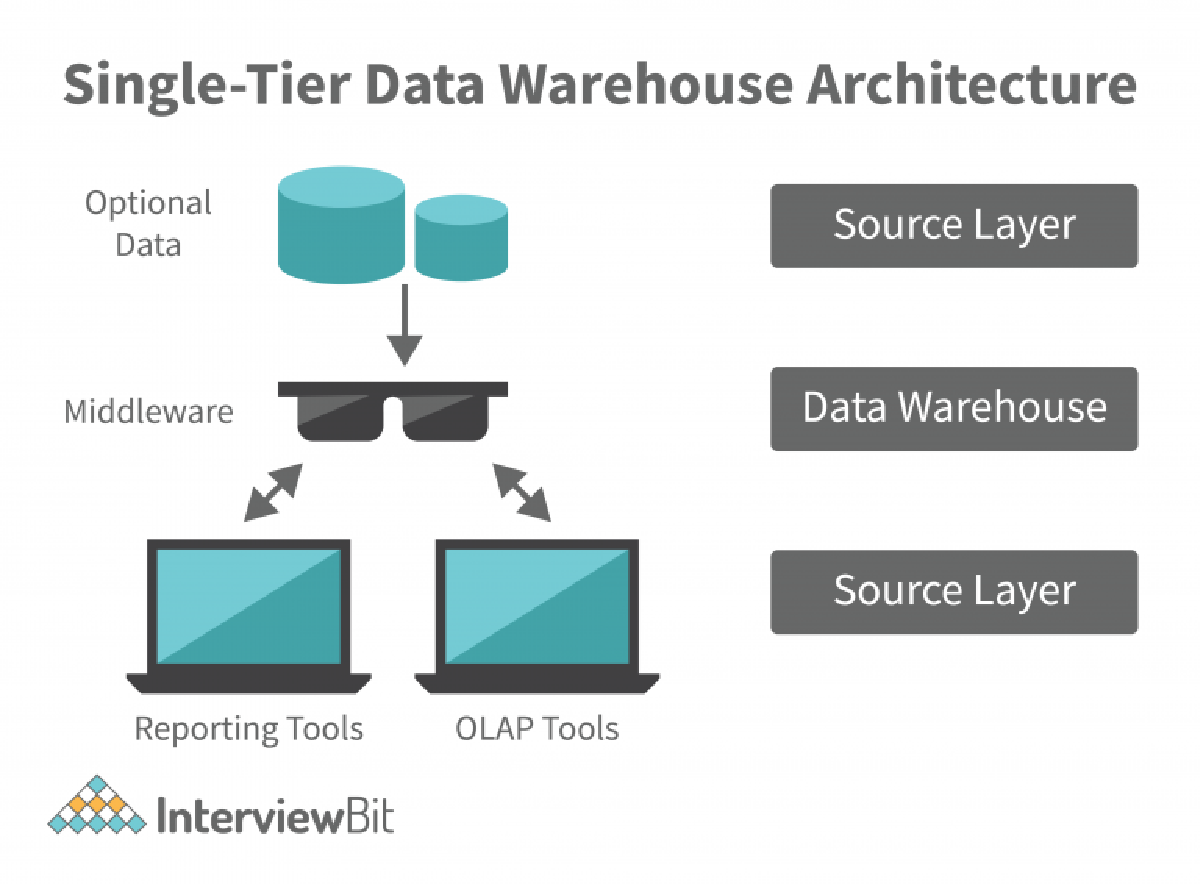
\includegraphics[width=0.7\linewidth]{figure/capitolo_2/DW - Single Tier Architetcure.pdf}
    \caption{Architettura di un Data Warehouse a singolo livello}
    \label{fig:DW-Single_Tier_Architecture}
    \end{figure}
    \item \textbf{Architetture a doppio livello}. In un'architettura a due livelli il processo analitico è separato da un processo di logica di business, permettendo in questo modo un maggiore livello di controllo ed efficienza. Tale sistema fornisce una migliore comprensione dei dati e permette decisioni più informate. In questa architettura -- rappresentata nella Figura \ref{fig:DW - Double Tier Architetcure} viene aggiunto il livello di data warehouse e ciò permette alla stessa di descrivere un flusso dei dati suddiviso in quattro differenti fasi:
        \begin{enumerate}
            \item \textit{L'origine dei dati} è critica per l'integrità del DW. L'integrità dei dati memorizzati deve essere garantita poiché essa è la rappresentazione del grado di veridicità ed accuratezza dei dati registrati ed un data warehouse deve essere composto di dati che possano essere definiti affidabili.
            \item La \textit{fase di staging dei dati} è un punto chiave del processo ETL e può ridurre significativamente il tempo necessario per la sua esecuzione. L'operazione di ETL è estremamente fondamentale per un processo di data warehousing e per questo motivo migliorare il più possibile tale ambito.
            \item I \textit{metadati} sono un elemento di grande rilevanza in un data warehouse poiché corrispondono alle informazioni che aiutano un amministratore del sistema a decidere le logiche da applicare sulla gestione dei dati. Tali informazioni, permettono di mantenere una coerenza della logica di gestione applicata all'interno del DW, che è un valore critico per una eventuale analisi o report sviluppato su tali dati.
            \item La \textit{profilazione dei dati}\footnote{La \textit{profilazione dei dati} è il processo di esame dei dati disponibili da una fonte di informazioni esistente e la raccolta di statistiche o riepiloghi formativi su tali dati.} è l'ultimo livello poiché si occupa di convalidare l'integrità dei dati e gli standard di una possibile presentazione. Esso comprende anche analisi avanzate come la generazione di rapporti in tempo reale e batch e le visualizzazioni.
        \end{enumerate}
    \begin{figure}[H]
    \centering
    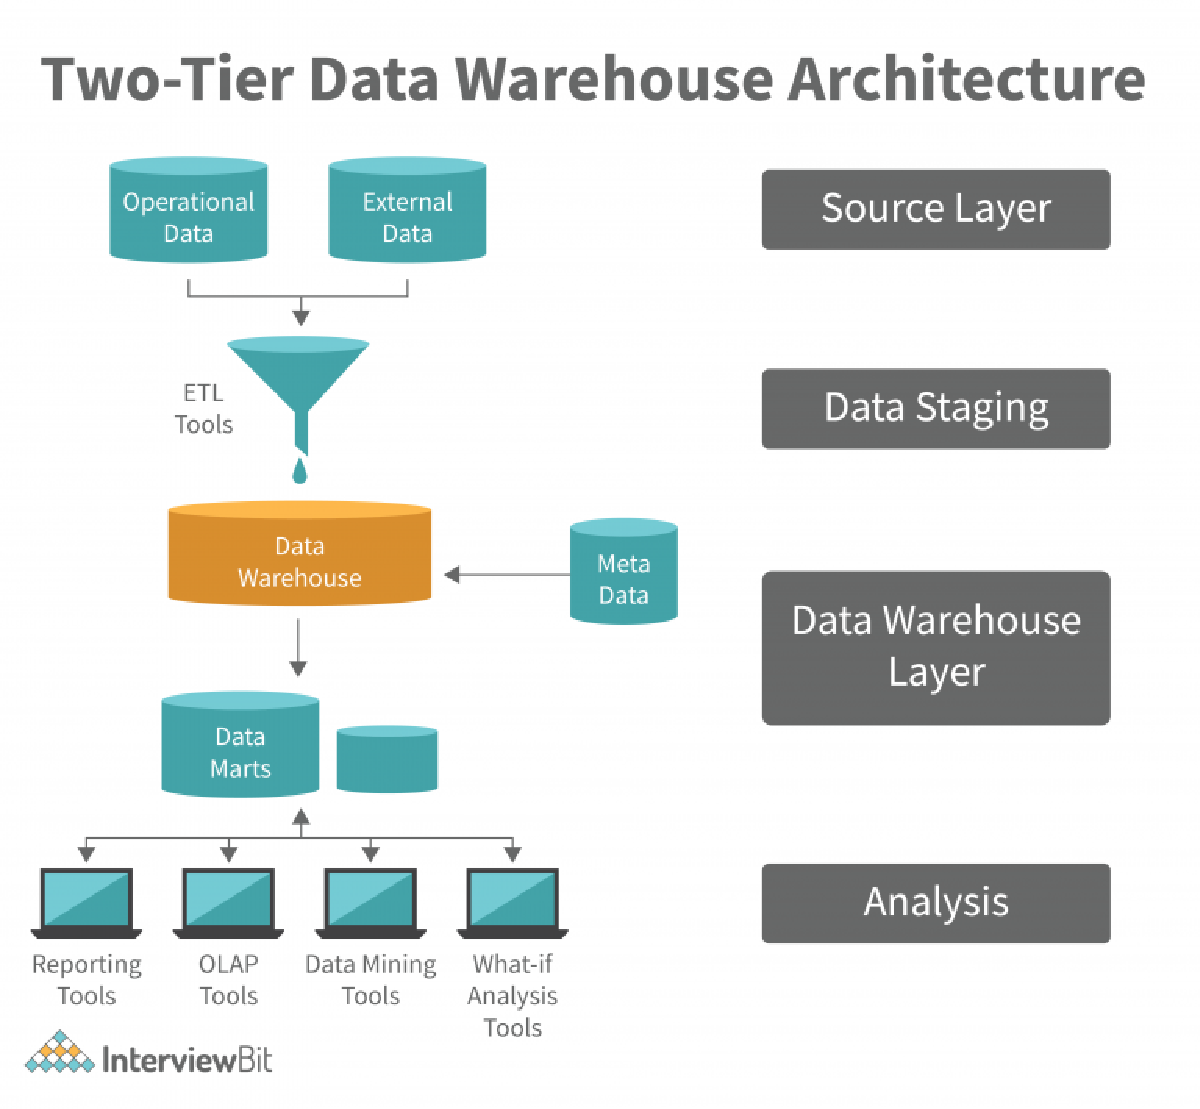
\includegraphics[width=0.7\linewidth]{figure/capitolo_2/DW - Double Tier Architetcure.pdf}
    \caption{Architettura di un Data Warehouse a doppio livello} 
    \label{fig:DW - Double Tier Architetcure}
    \end{figure}
    \item \textbf{Architetture a triplo livello}. Una architettura a tre livelli -- rappresentata nella Figura \ref{fig:DW - Triple Tier Architetcure} aggiunge al livello di origine quello di conciliazione e di data warehouse. Il principale svantaggio del livello di conciliazione è che non sia possibile ignorare completamente i problemi dei dati prima che questi vengano effettivamente conciliati. Più precisamente, il focus principale di chi si occupa di questo compito corrisponde a verificare l'integrità, l'accuratezza e la coerenza dei dati. Ogni volta che si verifica una modifica nei dati, viene eseguito uno strato aggiuntivo di revisione ed analisi di quest'ultimi per garantire che non ne siano stati inseriti nuovi errati. Questa architettura è molto affine a sistemi con un ciclo di vita lungo.
    \begin{figure}[H]
    \centering
    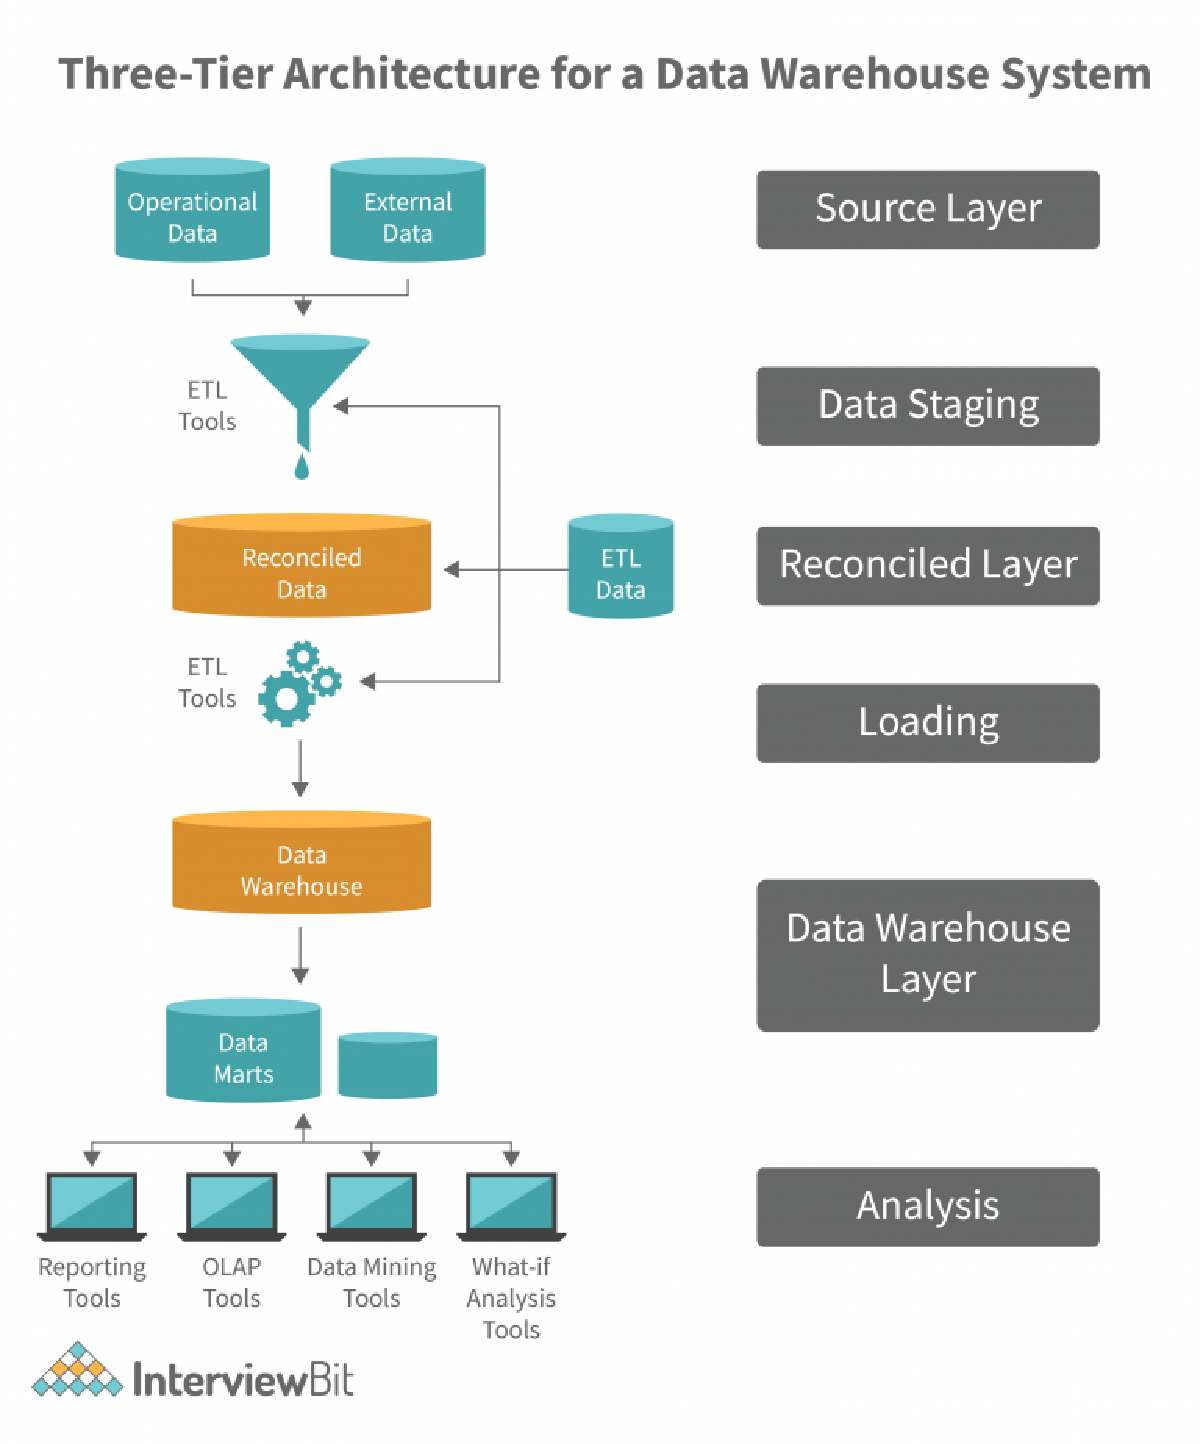
\includegraphics[height=0.75\linewidth]{figure/capitolo_2/DW - Triple Tier Architetcure.pdf}
    \caption{Architettura di un Data Warehouse a triplo livello} 
    \label{fig:DW - Triple Tier Architetcure}
    \end{figure}
\end{itemize}

\subsection{Processo ETL (Extract, Transform, Load)}

In precedenza è stato fatto riferimento alla procedura fondamentale per i data warehouse di raccolta, organizzazione e gestione dei dati dalle varie sorgenti a cui si fa riferimento. Il compito di questa procedura è rendere i dati di un'azienda disponibili recuperandoli da molteplici fonti, ripulire e trasformare tali dati in modo da evitare l'inflazionamento delle informazioni reperibili da eventuali analisi da parte di dati errati o non logicamente corretti. Alcuni esperti del settore hanno indicato che lo sforzo impiegato per questa procedura all'interno di un progetto di data warehousing è pari ad un valore tra il 60\% e l'80\% del totale. Questo perché tale procedura di recupero e gestione dei dati permette di avere informazioni utili/strategiche all'interno del DW. Se questo procedimento non viene fatto correttamente, i dati originari non avrebbero alcuna utilità per la fase di interrogazione ed analisi degli stessi, rendendo l'uso del sistema di data warehousing inutile \cite{researchgate_etl_process}.

Tale procedura si basa su tre operazioni principali, ovvero \cite{sciencedirect_data_warehouse_model}:
\begin{itemize}
    \item \textbf{Estrazione} (\textit{Extract}). Tale operazione è responsabile per il recupero dei dati dai sistemi di origine. Ogni fonte di dati ha un insieme di caratteristiche differenti che devono essere gestite correttamente per permettere un'estrazione efficiente. Per questo motivo, tale fase deve integrare efficacemente sistemi che utilizzano piattaforme, database, sistemi operativi o protocolli diversi tra loro.
    \item \textbf{Trasformazione} (\textit{Transform}). Tale operazione è responsabile di effettuare pulizia ed adattamento (mappatura, trasformazioni, ecc.) dei dati in questione per ottenere dei dati in formati precisi in modo che siano corretti, completi, coerenti e assolutamente non ambigui. Le regole applicate per svolgere ciò dipendono dalle politiche aziendali e da quale tipologia di dati (formati e ambiti trattati) bisogna gestire. Tutte le regole applicate sono descritte nel modulo dei metadati così da poterne tenere traccia.
    \item \textbf{Caricamento} (\textit{Load}). Tale operazione è responsabile del salvataggio dei dati recuperati all'interno del sistema di data warehouse. Naturalmente, essendo molto probabile che la quantità di dati da gestire sia elevata, tale fase deve utilizzare tecniche di ottimizzazione che permettano di aumentare le prestazioni così da permettere agli utenti finali dia vere a disposizione il prima possibile i dati di cui necessitano.
\end{itemize}

\begin{figure}[H]
    \centering
    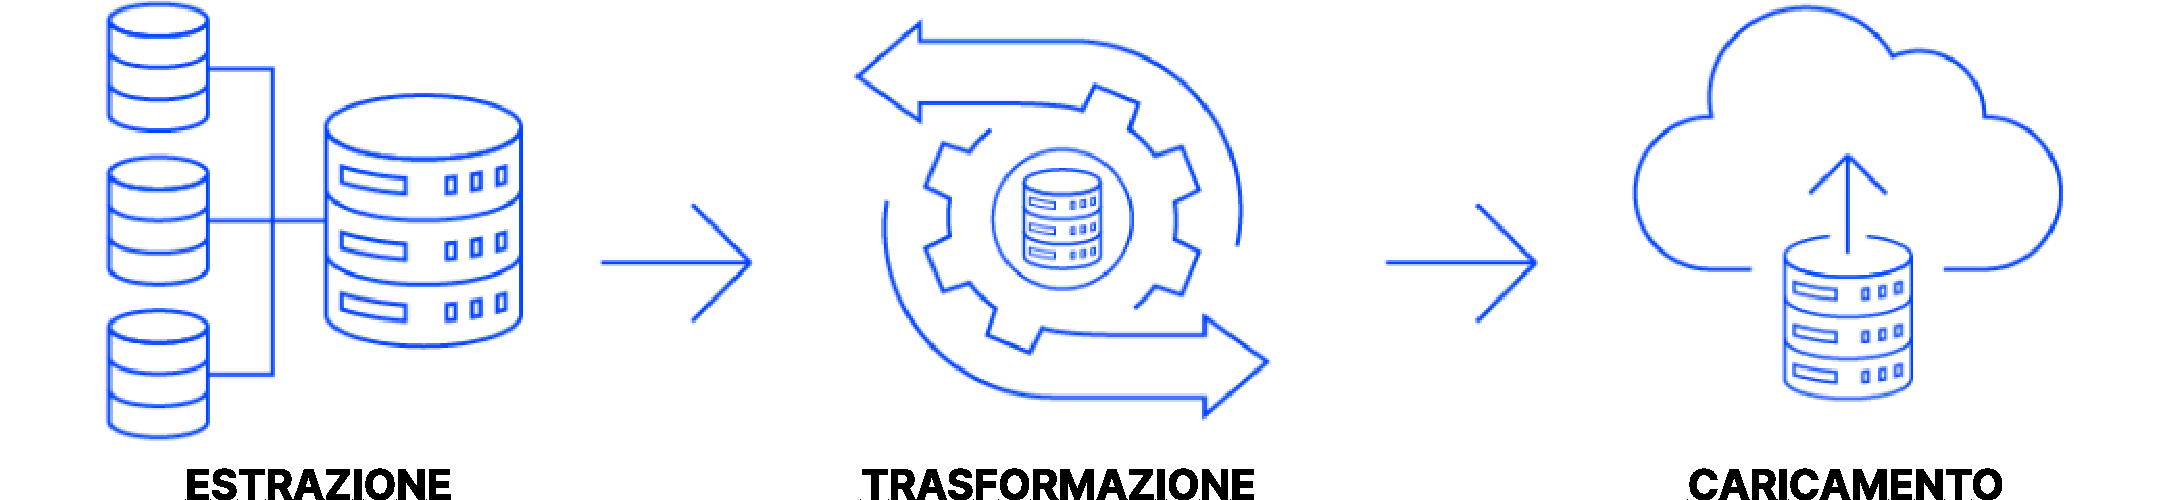
\includegraphics[width=1\linewidth]{figure/capitolo_2/ETL Process.pdf}
    \caption{Processo di ETL}
    \label{fig:ETL Process}
\end{figure}

\subsection{I Metadati}

Nel mondo dei dati, non esistono solo le informazioni essenziali riportate dai dati stessi, ma anche altre informazioni “secondarie” che permettono di descrivere, spiegare, localizzare o contestualizzare le informazioni “principali” dei dati; anche questi sono dei dati, più precisamente prendono il nome di \textit{metadati} (a volte anche definiti grossolanamente come “dati su dati”). Il termine \textbf{metadata} si riferisce alle informazioni che integrano i dati reali. Spesso, i metadati forniscono maggiori dettagli sul contesto del contenuto di un file o danno istruzioni come gestire i dati stessi\footnote{\textit{URL Fonte}: https://tinyurl.com/te2az9x3}.

Una volta spiegati cosa sono, è facile comprendere come questi siano una componente importante nel mondo del data warehousing. Una gestione coerente dei metadati permette una riduzione degli sforzi amministrativi e un miglioramento dello sfruttamento del sistema stesso. Una gestione corretta richiede che essi vengano recuperati e memorizzati all'interno di un apposito repository consultabile sia dai vari gruppi di utenti, al fine di essere utilizzato come documentazione da consultare per completare efficientemente i propri compiti, che da prodotti software, come ulteriore risorsa di informazioni e dati da sfruttare per valorizzare i propri lavori. L'esistenza di un singolo repository per la gestione di tutti i tipi di metadati all'interno di un'azienda ne consente una gestione centralizzata, uniforme, coerente e di facile accesso a qualsiasi tipologia di consumatore \cite{metadata_standards}.

\subsection{I Data Mart}

Un \textbf{Data Mart} (\textit{DM}) è archivio dati progettato per contenere dati di uno specifico ambito/argomento. In altre parole, è possibile definire i data mart come delle partizioni del data warehouse complessivo. Essendo una specializzazione di un DW, un DM è meno costoso ed impegnativo in termini di tempi di gestione e ricerca rispetto al sistema totalitario. Pertanto, in generale si può dire che un data mart integra e migliora la funzionalità di un data warehouse più grande.

Come sopracitato i data mart si focalizzano su determinati ambiti o funzionalità, perciò i dati caricati al loro interno che soddisfano tali caratteristiche possono arrivare dallo stesso data warehouse di cui fanno parte, una fonte esterna o altro. In base alla fonte da cui questi dati vengono recuperati è possibile categorizzare un data mart in due modi differenti \cite{itl_data_warehousing_and_mining}:

\begin{itemize}
    \item \textit{Data mart dipendente}. Il data mart è composto recuperando i dati da un data warehouse principale già esistente. Un processo di ETL con un data mart dipendente è semplificato poiché i dati hanno già subito l'operazione di trasformazione per essere caricati nel DW da cui si stanno estraendo. Per questo motivo, il processo di ETL in questo caso è incentrato sull'identificare il sottoinsieme dei dati interessato per il relativo ambiente di richiesta. Questa tipologia è solitamente adoperata per ottenere prestazioni migliori, un controllo più efficiente, maggiore disponibilità e minori costi.
    \item \textit{Data mart indipendente}. Il data mart è composto recuperando i dati da fonti operative, o esterne oppure entrambe. A differenza dei data mart dipendenti, questa tipologia viene creata senza l'uso di un data warehouse principale di riferimento. Tuttavia, in questo caso il processo di ETL non viene semplificato, anzi viene aggravato della necessità di recuperare dati solo di un determinato ambito, complicando la query di ricerca ed estrazione. Questa tipologia ha il vantaggio di essere utile per piccoli gruppi di attività e soddisfa la maggior parte delle esigenze degli utenti ad un costo e tempistiche minori rispetto ad un sistema di data warehouse completo.
\end{itemize}

Di seguito è riportata una tabella riepilogativa –– che evidenzia i risultati dello studio\footnote{\textit{URL Fonte}: https://streamsets.com/blog/data-mart-vs-data-warehouse/}––  che spiega le differenze tra un data mart e un data warehouse:

\begin{longtable}{|p{4cm}|p{5cm}|p{5cm}|}
    \caption{Data Mart e Data Warehouse a confronto} \\
    \hline
    \textbf{Categoria} & \textbf{Data Mart} & \textbf{Data Warehouse}\\
    \hline
    \endfirsthead 
        
        Sorgente dati & Spesso poche fonti di dati, orientate al soggetto e contenenti dati specifici. & Sfruttano molte fonti di dati.\\
        \hline
        
        Costi e Grandezza & Entrambi bassi. & Entrambi molto alti.\\
        \hline
        
        Performance & Solitamente ha un'alta velocità, dovuta alla quantità limitata di dati. & Potrebbe avere problemi di prestazioni a causa delle loro grandi dimensioni.\\
        \hline
        
        Sicurezza & I dati sensibili possono essere omessi completamente. & È necessario adottare misure di sicurezza per proteggere i dati sensibili.\\
        \hline
        
        Facilità di implementazione & Può essere abbastanza veloce perché i dati sono pochi. & Potrebbe necessitare di molto tempo, anche anni, data la grande complessità.\\
        \hline
        
        Longevità & Solitamente rimossi dopo che lo scopo per il quale sono stati costruiti è stato completato. & Può estendersi per tutta la vita dell'organizzazione.\\
    
    \hline
\end{longtable}

\subsection{I Data Lake}

In precedenza è stato fatto riferimento al termine \textit{data lake}, più precisamente un \textbf{Data Lake} si riferisce a un repository di archiviazione estremamente scalabile contenente una vasta quantità di dati grezzi nel loro formato nativo fino a quando non sia necessario, oltre a sistemi di elaborazione in grado di acquisire dati senza compromettere la struttura dei dati. I data lake sono tipicamente progettati per gestire grandi volumi di dati non strutturati che vengono recuperati rapidamente e da cui vengono estratte ulteriori informazioni. Proprio per questo motivo i data lake adoperano applicazioni di analisi dinamiche, che sappiano adattarsi ai diversi formati di dati archiviati \cite{sciencedirect_data_lake}.

Nella seguente Figura \ref{fig:Data Lake Life Cycle} è raffigurato il ciclo di vita dei dati all'interno di un sistema di data lake. Questo schema ad alto livello ci permette di comprendere che mentre i dati confluiscono in determinato punto di acquisizione di un Data Lake, i corrispondenti metadati vengono recuperati e gestiti insieme alla relativa tracciabilità, provenienza e aspetti di sicurezza dei dati, durante il loro ciclo di vita \cite{data_lake_for_enterprices}.

\begin{figure}[H]
    \centering
    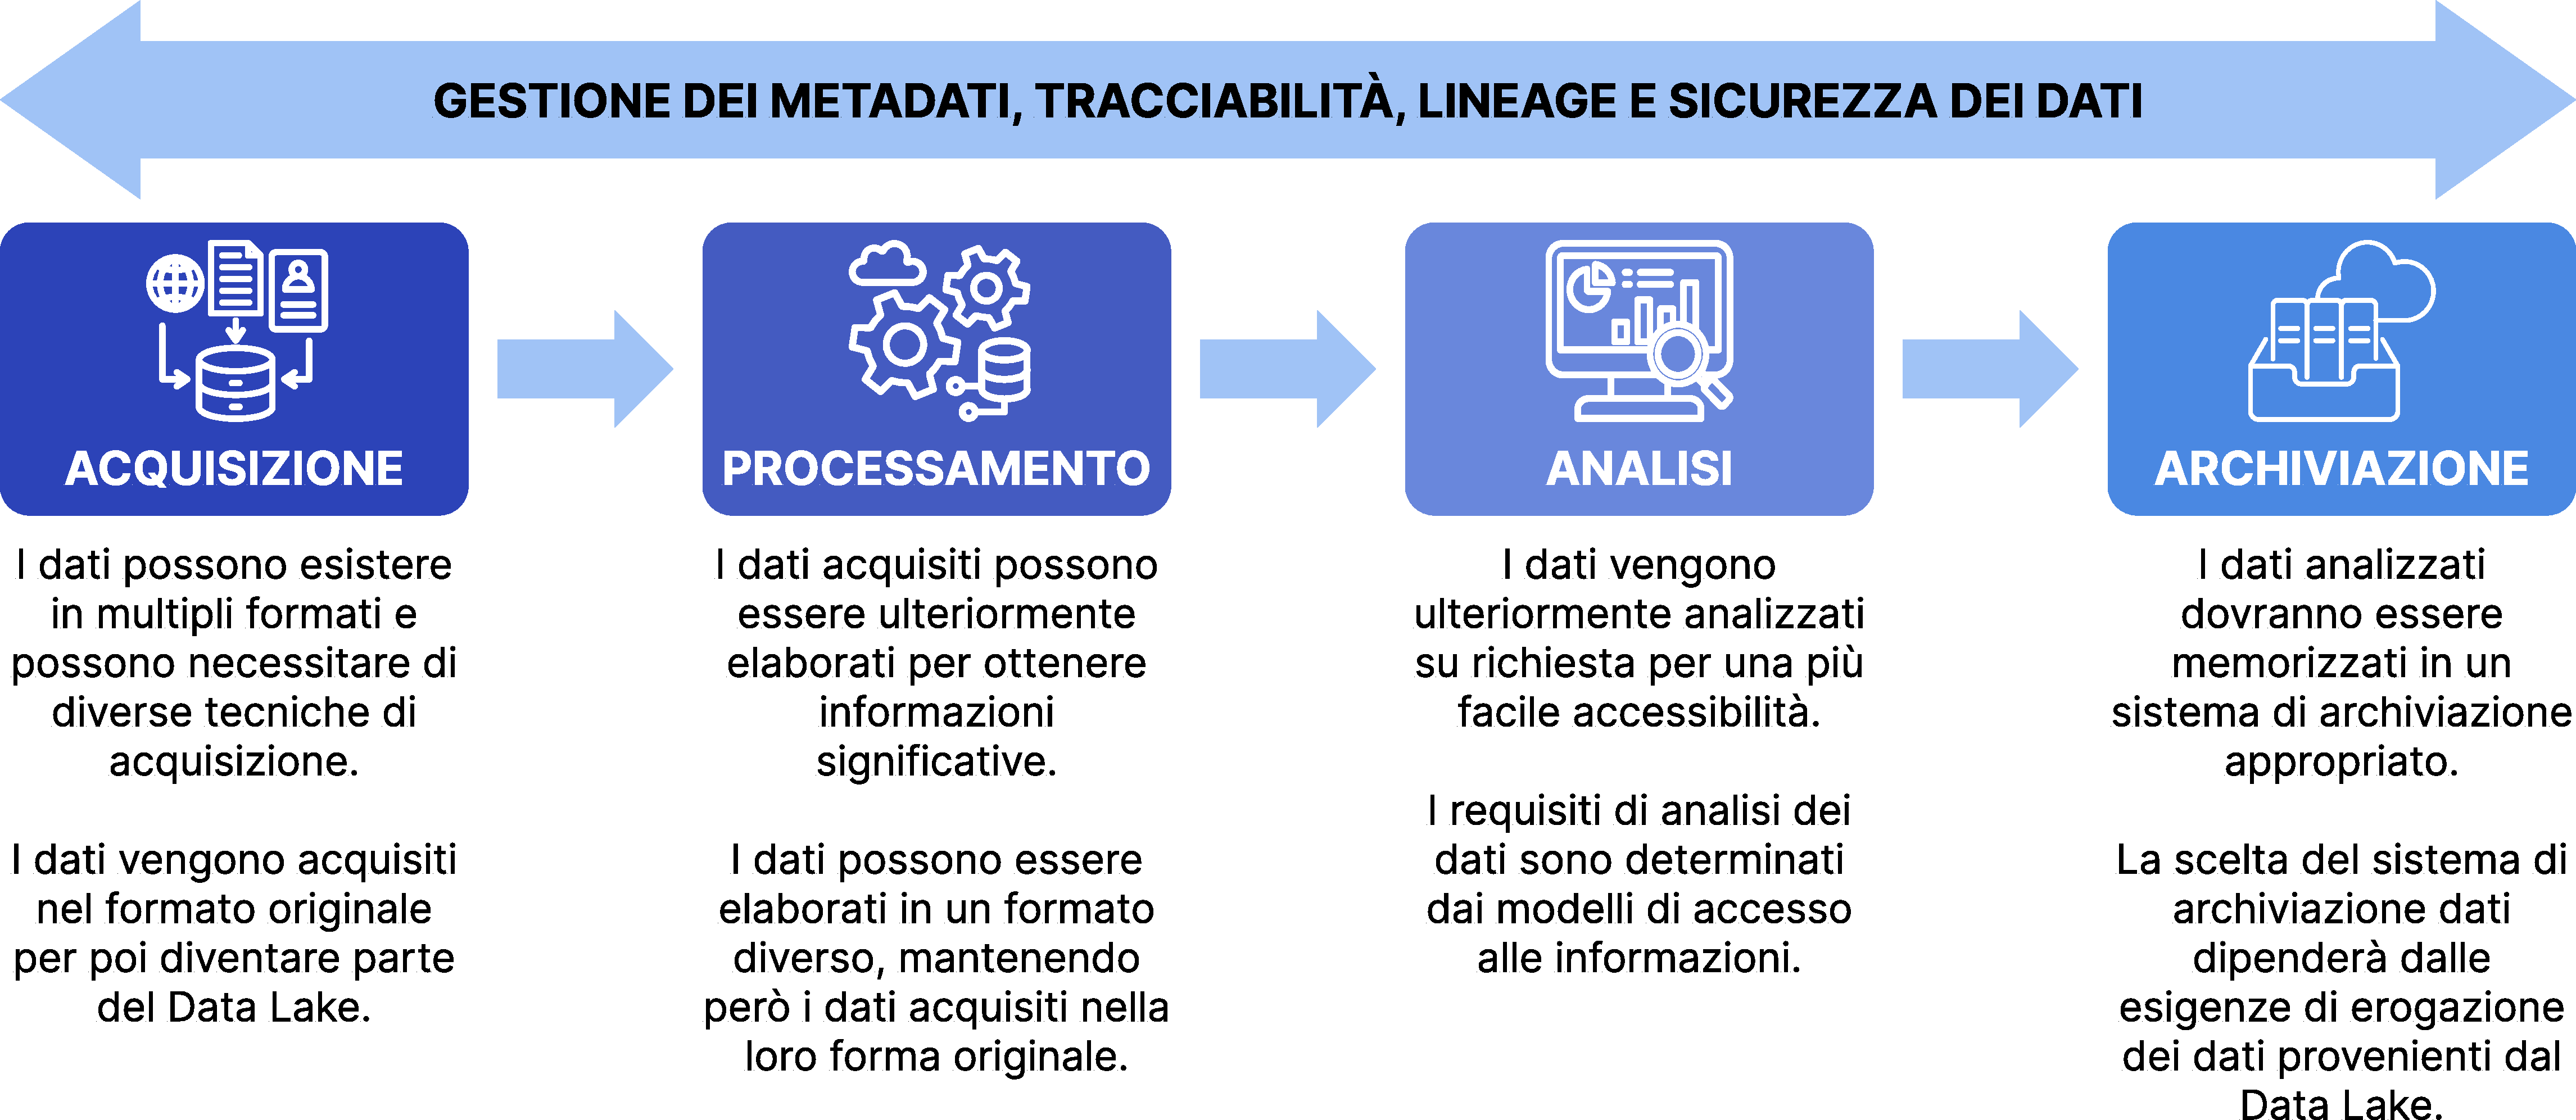
\includegraphics[width=1\linewidth]{figure/capitolo_2/Data Lake Life Cycle.pdf}
    \caption{Ciclo di vita dei dati nei Data Lake}
    \label{fig:Data Lake Life Cycle}
\end{figure}

Originariamente i data lake sono stati creati per sopperire all'incapacità dei data warehouse di gestire i volumi crescenti, la velocità e l'ampia serie di Big Data. I data lake, anche se più lenti dei DW, sono più economici poiché non necessitano delle operazioni di trasformazione. Data la mancanza di necessità di definire degli obiettivi di business da applicare sui dati, hanno tantissimi possibili casi di utilizzo. Tuttavia, i due principali casi di utilizzo comprendono l'esplorazione della data science e le attività di ripristino e backup dei dati\footnote{\textit{URL Fonte}: https://www.ibm.com/topics/data-architecture}.

Di seguito è riportata una tabella riepilogativa dei risultati ottenuti nello studio\footnote{\textit{URL Fonte}: https://aws.amazon.com/data-warehouse/}, che spiega le differenze tra un data lake e un data warehouse:

\begin{longtable}{|p{4cm}|p{5cm}|p{5cm}|}
    \caption{Data Lake e Data Warehouse a confronto}
    \label{tab:data_lake_vs_data_warehouse} \\
    \hline
    \textbf{Caratteristiche} & \textbf{Data Lake} & \textbf{Data Warehouse}\\
    \hline
    \endfirsthead 

    Dati & Tutti i dati, compresi strutturati, non strutturati e semi-strutturati. & Dati relazionali da sistemi transazionali, database e applicazioni aziendali.\\
    \hline
    Schema & Creato al momento dell'analisi. & Spesso progettato prima dell'implementazione, ma può essere creato anche al momento dell'analisi.\\
    \hline 
    Prezzo/Prestazioni & I risultati delle query diventano più veloci utilizzando l'archiviazione a basso costo e il disaccoppiamento dei processi di elaborazione e archiviazione. & Risultati delle query più rapidi utilizzando uno storage locale.\\
    \hline
    Qualità dei dati & Qualsiasi dato curato e non. & Dati estremamente curati che fungono da versione veritiera centrale.\\
    \hline
    Utenti & Analisti aziendali, data scientist, sviluppatori ed ingegneri di dati. & Analisti aziendali, data scientist e sviluppatori di dati.\\
    \hline    
    Analisi & Machine learning, analisi esplorativa, rilevamento di dati, streaming, analisi operativa, Big Data e profilazione. & Reporting in batch, BI e visualizzazioni.\\
    \hline
\end{longtable}

\section{Analisi dei Dati}

Se il capitolo \ref{ch:Introduzione} ci ha permesso di comprendere quanto i dati siano importanti e come siano diventati tali, con l'attuale sono stati spiegati largamente i concetti di \textit{Big Data} e \textit{Data Warehousing} permettendoci di comprendere quali sono le operazioni, le infrastrutture e i modelli necessari alla loro gestione. Tutto ciò si raggruppa in un singolo macro ambito, ovvero quello dell'\textit{analisi dei dati}.

Più precisamente, l'\textbf{analisi dei dati} (o \textit{Data Analytics}) è il processo grazie al quale vengono ricavate le informazioni dai dati, precedentemente estratti, trasformati e centralizzati, per permettere di scoprire, analizzare e comprendere dei possibili schemi (o modelli) nascosti, relazioni, tendenze e anomalie presenti al loro interno. L'obiettivo dell'analisi dei dati è quindi identificare informazioni utili, suggerire conclusioni e aiutare a prendere decisioni accurate\footnote{\textit{URL Fonte}: https://www.talend.com/resources/what-is-data-analytics/}.

\subsection{Tipologie di Analisi}
L'analisi dei dati viene utilizzata per aumentare la produttività e le entrate con una riduzione dei costi in qualsiasi settore. Essa permette di dare un senso a grandi volumi di dati la cui forma grezza è priva di un modello specifico data la loro probabile varietà. Raccogliere e archiviare una quantità così elevata di dati acquisisce valore solamente se ben utilizzati e l'analisi è uno dei migliori modi per farlo \cite{researchgate_big_data_analytics}.
Tuttavia, data l'eterogeneità si dei dati che degli ambiti di utilizzo, è necessario applicare tecniche di analisi differenti dipendentemente dalle proprie necessità. Proprio per questo motivo è possibile suddividere i modelli analitici ––raffigurati in Figura \ref{fig:Analytics Models}\footnote{\textit{URL della Figura}: https://tinyurl.com/3j6u4f9j}–– in quattro tipologie \cite{big_data_analytics_harnessing_data_for_new_business_models}:

\begin{enumerate}
    \item \textbf{Analisi Descrittiva}. Risponde alla domanda “Cosa sta accadendo?”. Corrisponde alla fase preliminare dell'elaborazione dei dati che crea un insieme di dati storici. In altre parole, gestisce ciò che accade in tempo reale e ciò che è accaduto in passato, così da comprendere le cause dei successi e fallimenti avvenuti in passato e conoscere gli eventuali ambiti su cui dover approfondire le proprie conoscenze date le tendenze attuali.
    \item \textbf{Analisi Diagnostica}. Risponde alla domanda “Perché è avvenuto?”. Essa esamina le informazioni passate per conoscere come, cosa e perché un evento è successo. In altre parole, il proprio scopo è quello di scoprire eventuali informazioni che permettano di identificare la causa principale di un problema e quindi i fattori che hanno causato direttamente o indirettamente un avvenimento.
    \item \textbf{Analisi Predittiva}. Risponde alla domanda “Cosa è probabile che accada?”. Questa analisi adopera i dati passati e presenti per prevenire cosa possa accadere in futuro, fornendo le probabilità associate all'evento in questione. Proprio a questo scopo vengono utilizzati sistemi di Data Mining associati a modelli specifici di intelligenza artificiale per svolgere l'analisi e creare i possibili scenari che potrebbero generarsi.
    \item \textbf{Analisi Prescrittiva}. Risponde alla domanda “Cosa si dovrebbe fare?”. Si dedica a riconoscere quale sia l'azione più corretta da intraprendere. Sfruttando i dati prevenienti dalle analisi precedentemente elencate, cerca di trovare la soluzione migliore tra le varie possibili. Essa va oltre la previsione dei risultati futuri, suggerendo anche i benefici dell'azione, secondo le previsioni generate, e mostrando al decisore le implicazioni di ciascuna scelta.
\end{enumerate}

\begin{figure}[H]
    \centering
    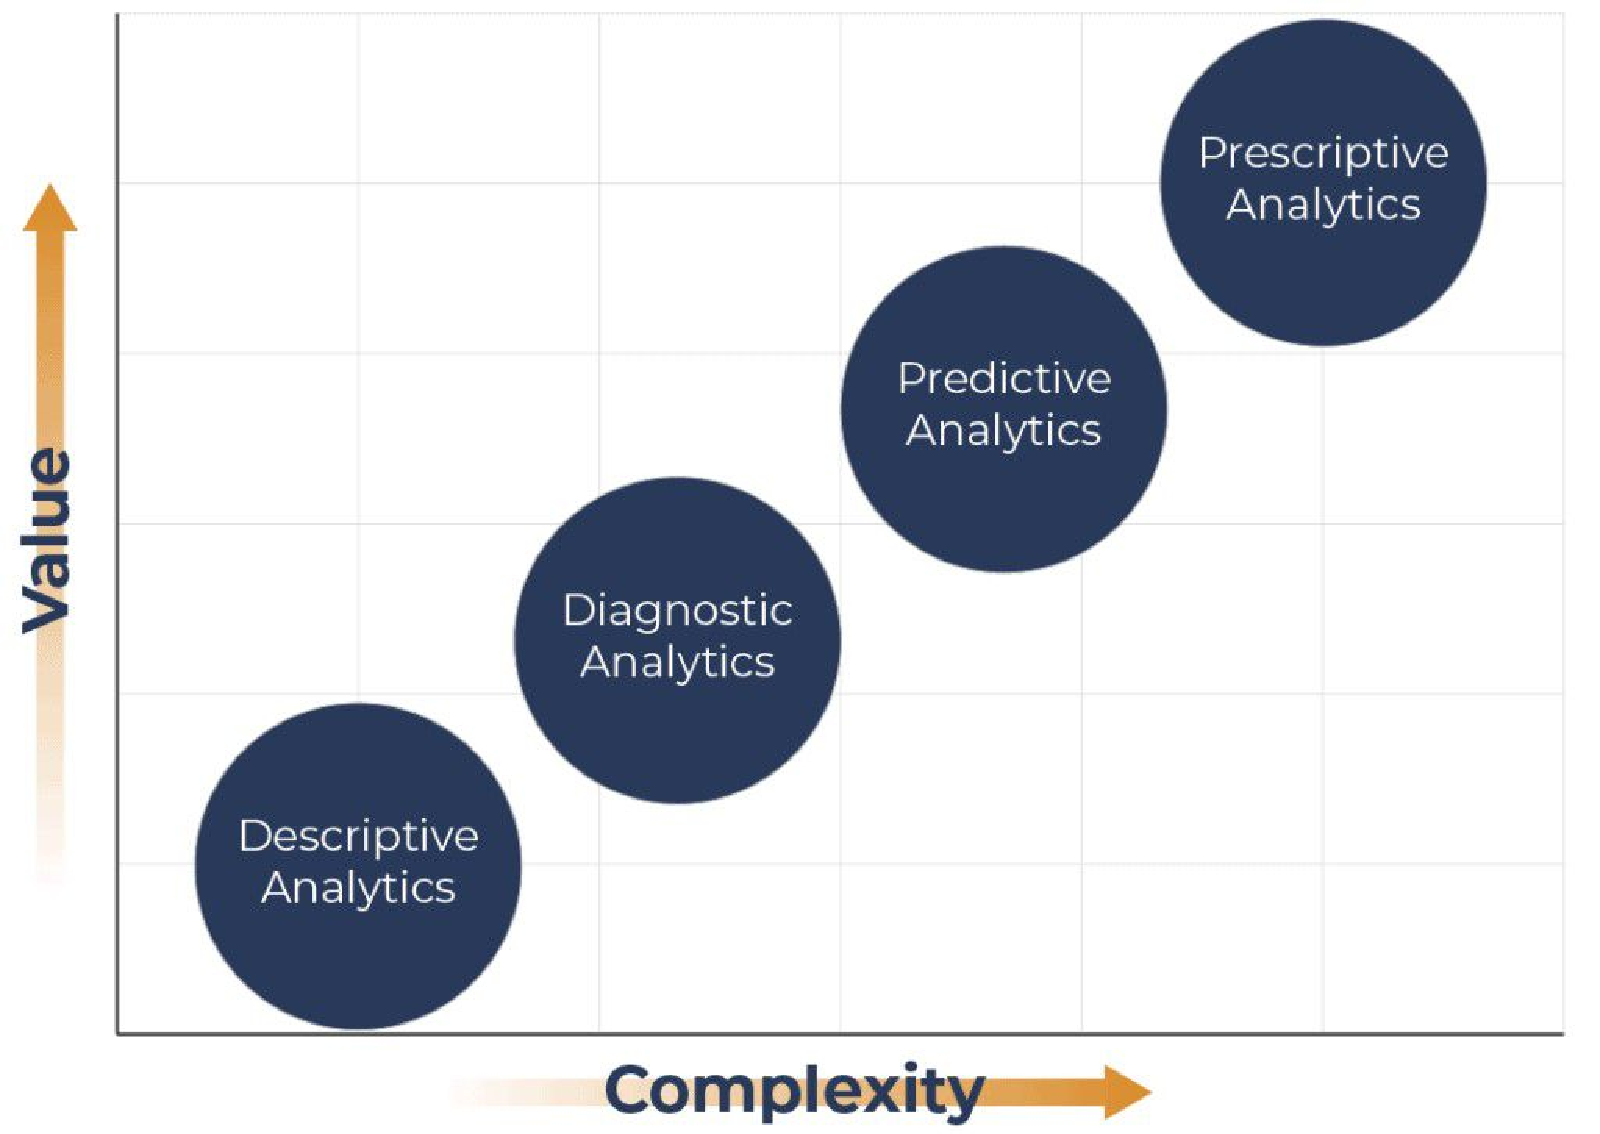
\includegraphics[width=0.75\linewidth]{figure/capitolo_2/Analytics Models.pdf}
    \caption{Tipologie di analisi dei dati}
    \label{fig:Analytics Models}
\end{figure}

\subsection{I Sistemi di Supporto alle Decisioni}

La rapida crescita di dati e quindi il relativo compito di doverli gestire e sfruttare al meglio ha portato ad avere una sempre maggiore necessità di supporto per la comprensione ed analisi degli stessi. Sono stati molti gli studi a riguardo che hanno riscontrato che le soluzioni prodotte dai decision maker sono al di sotto del loro possibile potenziale, poiché essi non sono in grado di assimilare l'elevato numero di informazioni per poter svolgere il proprio compito. Per sopperire a tale problema, sono stati ideati dei \textit{sistemi di supporto alle decisioni}, o \textit{Decision Support Systems} (\textit{DSS}), ovvero strumenti che assistono direttamente i responsabili delle decisioni esecutive nel proprio lavoro semplificando le informazioni da dover sfruttare.

La maggior parte delle ricerche sui DSS adotta uno dei seguenti concetti \cite{mit_keen_dss}:

\begin{itemize}
    \item I DSS sono definiti in base alla struttura del compito che devono affrontare.
    \item I DSS richiedono una strategia di progettazione che sia distintiva dipendentemente dalle tecniche di evoluzione.
    \item I DSS supportano i processi cognitivi dei singoli responsabili delle decisioni; la ricerca decisionale fornisce approfondimenti descrittivi sulla risoluzione dei problemi di gestione e teorie normative per definire come migliorarne l'efficacia.
    \item I DSS riflettono una strategia di implementazione per rendere i computer utili ai dirigenti; questa strategia si basa sull'uso di intermediari esperti, servizi reattivi e interfacce software user-friendly.
\end{itemize}

Più precisamente, un \textbf{Decision Support System} è un sistema informativo che aiuta un'azienda nel compito di svolgere attività decisionali che richiedono giudizio, determinazione e una determinata sequenza di azioni. Il DSS assiste la gestione di medio e alto livello dell'azienda che lo adotta analizzando enormi volumi di dati e accumulando informazioni che possono rendersi utili per la risoluzione di problemi o la presa di decisioni\footnote{\textit{URL Fonte}: https://tinyurl.com/228648zk}.

\begin{figure} [H]
    \centering
    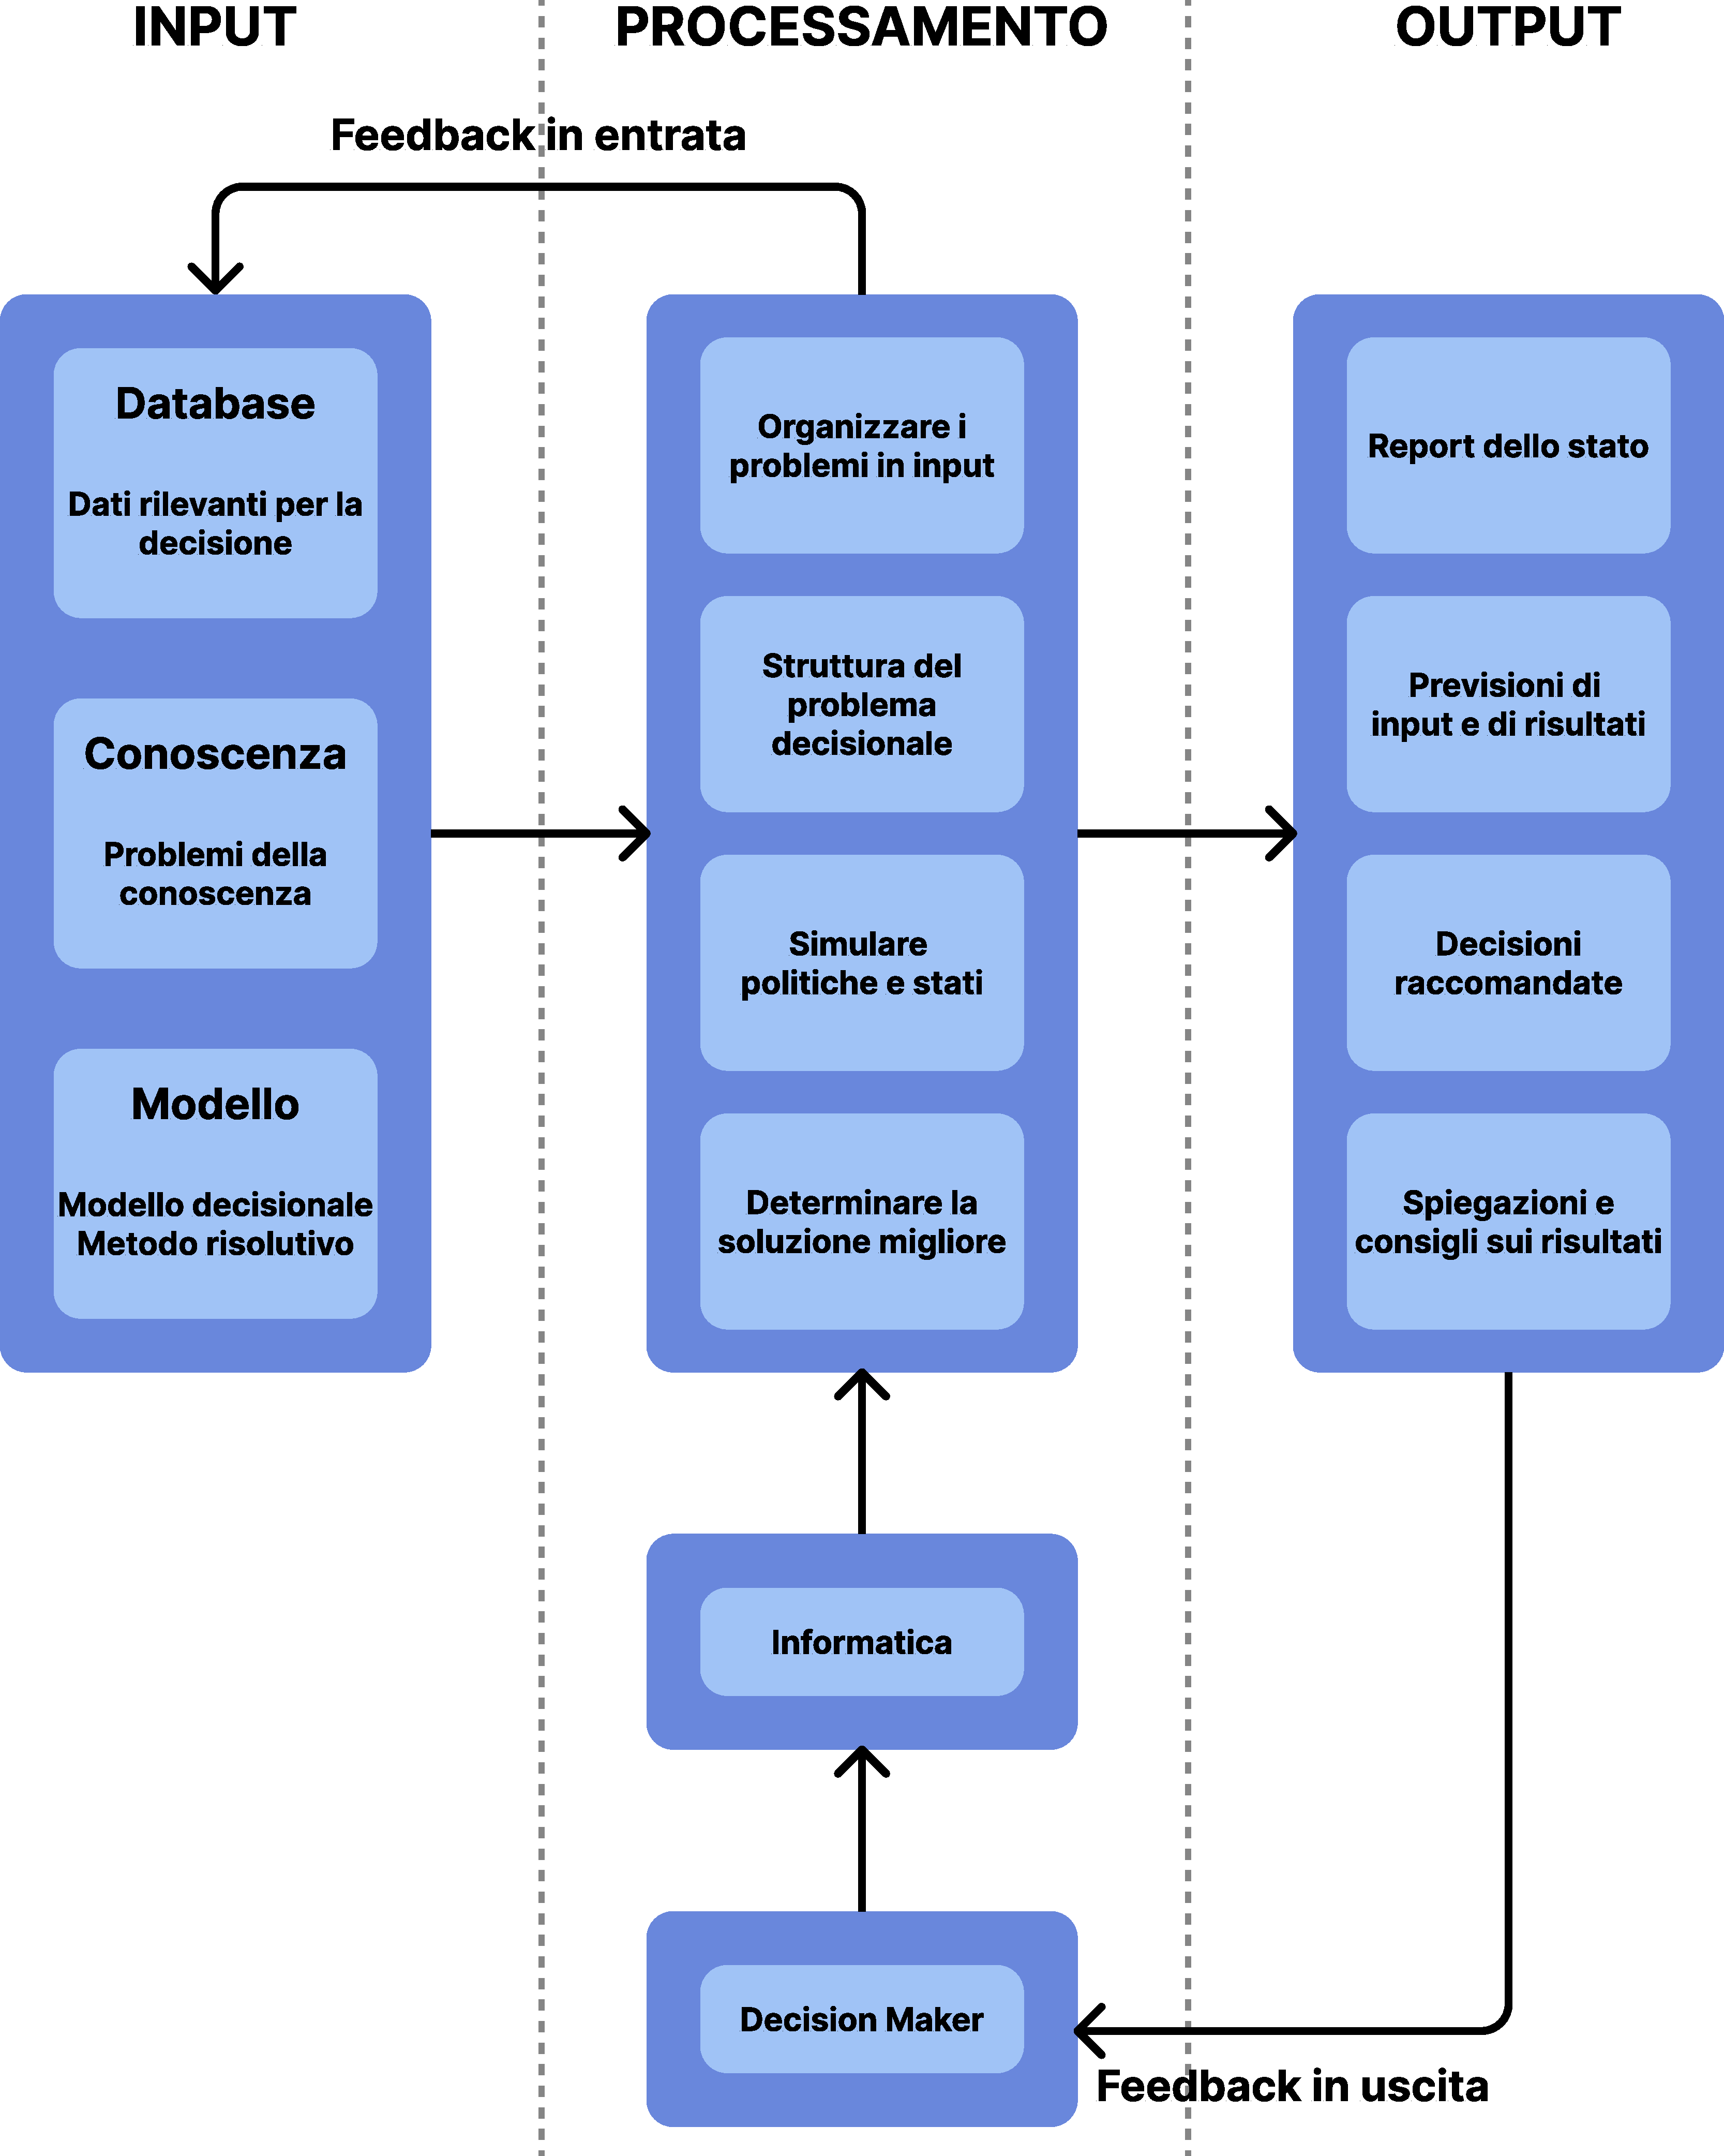
\includegraphics[height=1\linewidth]{figure/capitolo_2/Decision Support System Structure.pdf}
    \caption{Struttura di un sistema decisionale di supporto}
    \label{fig:Decision Support System Structure}
\end{figure}

\subsubsection{Le Caratteristiche}

Identificare le caratteristiche di un sistema decisionale di supporto non è un compito semplice data l'eterogeneità di quest'ultimi e degli ambiti in cui sono adoperati, tuttavia Turban e Aronson sono riusciti a ricapitolare quali siano le caratteristiche generali che li contraddistinguono \cite{dss_characteristics}.

\begin{itemize}
    \item Un DSS assiste i decision maker con la risoluzione di problemi semi e non strutturati facendo uso del giudizio umano e dei computer.
    \item Un DSS copre un ampio spettro di livello di gestione, dal mondo dirigenziale a quello operativo.
    \item Un DSS fornisce supporto indifferente ad individui singoli o gruppi.
    \item Un DSS facilita la presa di decisioni indipendenti e/o sequenziali che possono essere prese una o più volte.
    \item Un DSS gestisce tutte le fasi del processo decisionale, ovvero: raccolta di informazioni, progettazione, scelta ed implementazione.
    \item Un DSS copre un'ampia varietà di strumenti di analisi delle decisioni.
    \item Un DSS è adattabile e flessibile, permettendo agli utenti di aggiungere, modificare, eliminare o riorganizzare gli elementi base di cui si compone.
    \item Un DSS dovrebbe essere user-friendly.
    \item Un DSS ha l'obiettivo di migliorare l'efficacia della presa di decisioni (appropriatezza e qualità) anziché l'efficienza (il costo della presa di decisioni).
    \item Un DSS deve assistere e non sostituire un decision maker.
    \item Un DSS adotta diversi modelli di analisi per creare strategie diverse dipendentemente dalla situazione in cui si riscontra il problema.
    \item Un DSS dovrebbe essere in grado di fornire accesso a una varietà di fonti e formati differenti di dati.
    \item Un DSS può essere integrato con altri sistemi e può essere distribuito tramite tecnologie di rete e web per essere facilmente fruibile.
\end{itemize}

\subsubsection{Tipologie di DSS}

I sistemi di supporto alle decisioni possono essere suddivisi in differenti categorie dipendentemente dal principio su cui si basano, ovvero\footnote{\textit{URL Fonte}: https://www.techtarget.com/searchcio/definition/decision-support-system}:

\begin{itemize}
    \item \textit{Basati sui dati}. Questa tipologia basa il proprio supporto sui dati provenienti da database (interni o esterni) sfruttando principi di data mining per poterli analizzare e mostrare all'utente.
    \item \textit{Basati sui modelli}. Questa tipologia basa il proprio supporto sull'analizzare una situazione che corrisponda ad un modello/schema precedentemente definito in base ai requisiti dell'utente.
    \item \textit{Basati sulla comunicazione e DSS di gruppo}. Questa tipologia basa il proprio supporto sull'adottare diversi strumenti di comunicazione per consentire a più di una persona di lavorare su una specifica attività, con l'obiettivo di migliorare il valore delle scelte dovute ad una collaborazione tra più persone.
    \item \textit{Basati sulla conoscenza}. Questa tipologia basa il proprio supporto sull'utilizzo di una conoscenza aggiornata continuamente e gestita da un sistema di \textit{Knowledge Mangament} in modo da fornire informazioni sempre aggiornate e coerenti basate sulla conoscenza generale dell'azienda.
    \item \textit{Basati sui documenti}. Questa tipologia basa il proprio supporto sull'analisi dei documenti (interni o esterni) per rispondere a ricerche specifiche degli utenti e fornirgli le informazioni necessarie. 
\end{itemize}


\subsection{Business Intelligence (BI) e Business Analytics (BA)}
Come detto in precedenza, l'analisi dei dati è un termine ampio utilizzato per comprendere diverse metodologie di analisi dei dati. Tra queste metodologie due delle più rilevanti in ambito aziendale sono sicuramente la \textit{Business Intelligence} (\textit{BI}) e la \textit{Business Analytics} (\textit{BA}) (che inoltre, possono essere identificati anche come dei sistemi di supporto alle decisioni).

In termini generici, la BI e la BA si riferiscono all'infrastruttura collettiva, agli strumenti, alle applicazioni e ad altre risorse che generano dati e informazioni, che a loro volta valorizzano il modo in cui le aziende prendono decisioni, scoprono opportunità di guadagno e esaminano le proprie prestazioni.

Di seguito sono riportate delle spiegazioni generali per comprenderle meglio \cite{academiaedu_bi_and_ba}.

\begin{itemize}
    \item \textit{Business Intelligence}. La BI può essere descritta come un insieme di tecniche e strumenti che permettono l'acquisizione e la trasformazione di dati grezzi in informazioni importanti ed utili per fini aziendali. Tali tecniche sono in grado di gestire enormi quantità di dati (strutturati e in alcuni casi anche non) per permettere l'identificazione, lo sviluppo e la creazione di nuove opportunità strategiche utili alla compagnia.
    \item \textit{Business Analytics}. La BA può essere descritta come l'insieme di competenze, tecnologie e pratiche atte all'esplorazione continua e iterativa delle prestazioni passate di una compagnia al fine di ricavare possibili intuizioni ed aiutare quindi la pianificazione delle decisioni aziendali sulle future azioni da intraprendere. Tali tecniche si concentrano sullo sviluppo di nuove intuizioni e sulla comprensione delle prestazioni aziendali passate basandosi su dati e metodi statistici, in modo da migliorarne le future.
\end{itemize}